\chapter{Performance Evaluation}
\label{chp:perfeval}

\section{Predownload hit experiment}
In section \ref{section:predlsetup}, we have explained how we altered the program to measure swarms worth of investment. The program will periodically load all the \texttt{.torrent} file in a directory while also consider maximum number of active swarm. In a single load, program will start as much swarm as possible to fulfill the maximum amount of active swarm. The swarms will be loaded in batch with a fixed interval. \todo{Adding .torrent per seconds is unsignificant. Key is number of torrents in single session.}

We also limit the time needed for a swarm to be finished. If the time needed for \textit{predownloading} is more than 1 hour, we mark it as failed because of \textit{timeout}. In fact, the system will not wait until it is finished. It will stop when 1 hour threshold is reached. Maximum number of swarm in a source also contributes to \textit{predownload} time. The larger the number, the more active connection and memory needed for storing the data in a single time. In a sense, it entirely possible it will affect all of those swarms and make it slower to finish the \textit{predownload}.

The program uses local directory, where the crawler stored \texttt{.torrent} file, as a source. After load the \texttt{.torrent} file, \textit{predownload} mechanism will be automatically started. First, it will download the first piece of a swarm. After it finished, as part of \textit{predownload} mechanism, the system will look for several other rarest pieces while collecting information on the swarm. With limited attempts, if the rarest pieces could not be found, it will discard the swarm and marked as failed to \textit{predownload}. 

If a swarm is successfully downloaded, we also observe the peer that has been discovered. We put two checkpoints of peer discovery. First is when the swarm just finished its \textit{predownloading}. At this point, discovered peers are obtained along with the \textit{predownloading}. Second checkpoint is after waiting period. This period is reserved as an idle time to collect more information of the swarm. A peer as a Web seed or http seed are excluded from the list. By doing this, we intend to evaluate the overall \textit{predownload} period and its timing mechanism.

In the figure \ref{fig:predownprecent}, it is shown the percentage of swarm that has been successfully \textit{predownloaded}. In this experiment, we inserted 100 swarm in one batch. The number of piece that need to be downloaded is 4. The number of maximum attempts to find rarest piece is 60 times with the interval of each attempt is 30 seconds. The finished swarms fall into two categories, it is either finished successfully or prematurely. As for the cause or prematurely finished, we divide it in three general category : timeout swarms, short swarms, and swarm with failure attempts.

\begin{figure}[h]
	\centering
	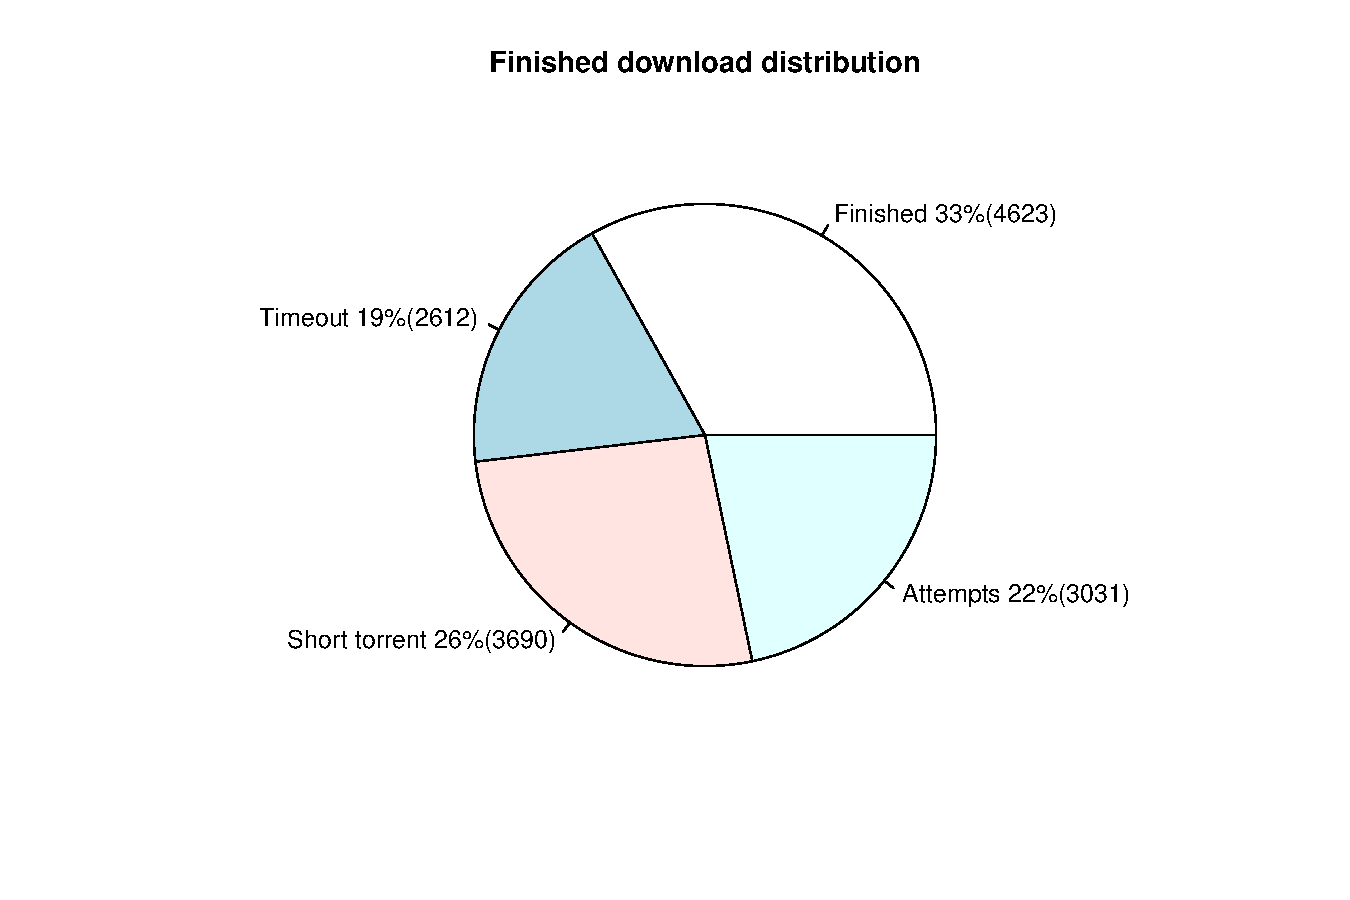
\includegraphics[width=0.7\textwidth]{pics/results/dpredown_t60i30.pdf}
	\caption{Predownload success percentage}
	\label{fig:predownprecent}
\end{figure}

\begin{figure}[h!]
	\begin{adjustwidth}{-2cm}{}
	\begin{subfigure}[t]{0.6\textwidth}
		\centering
		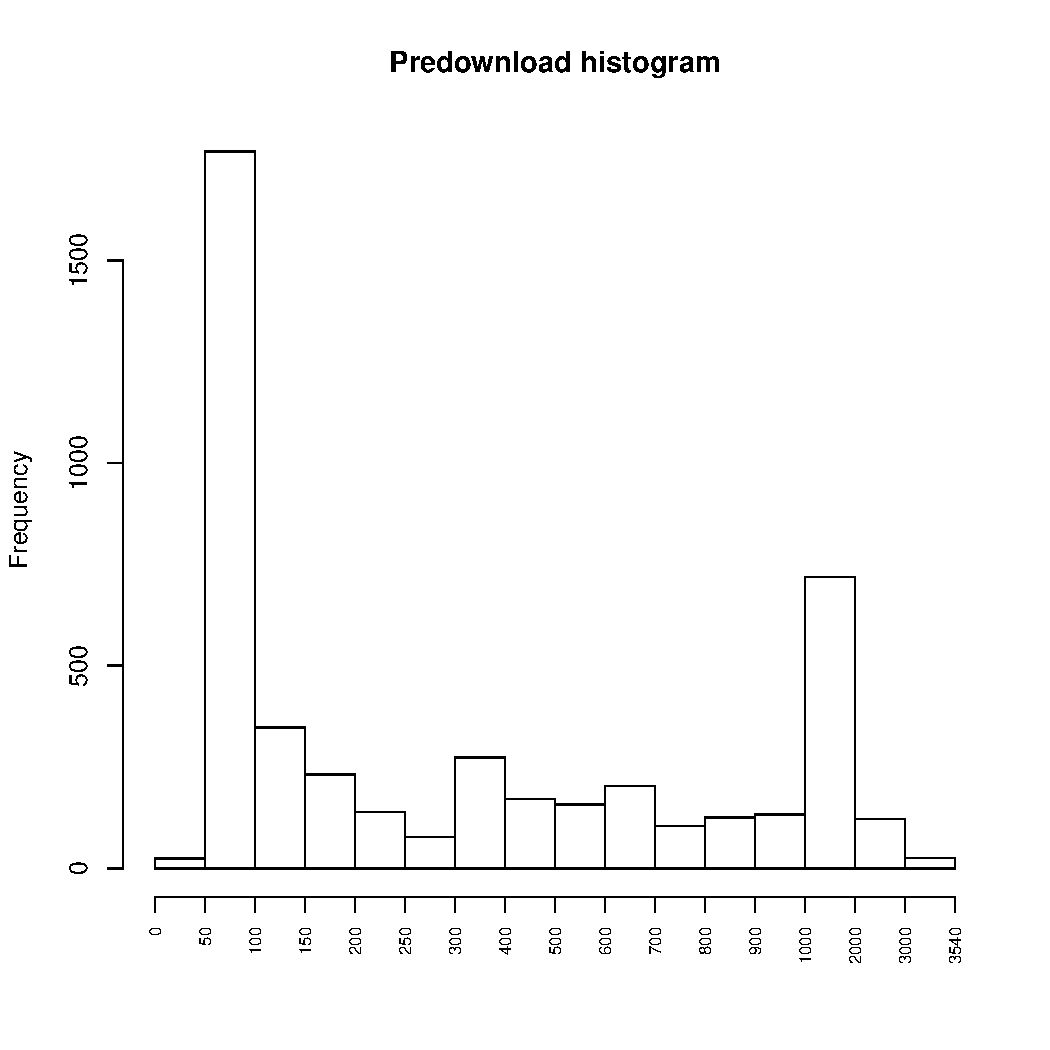
\includegraphics[width=\textwidth]{pics/results/hpredown_t60i30.pdf}
		\caption{Predownload distributed time}
		\label{fig:predownhist}
	\end{subfigure}
	~
	\begin{subfigure}[t]{0.6\textwidth}
		\centering
		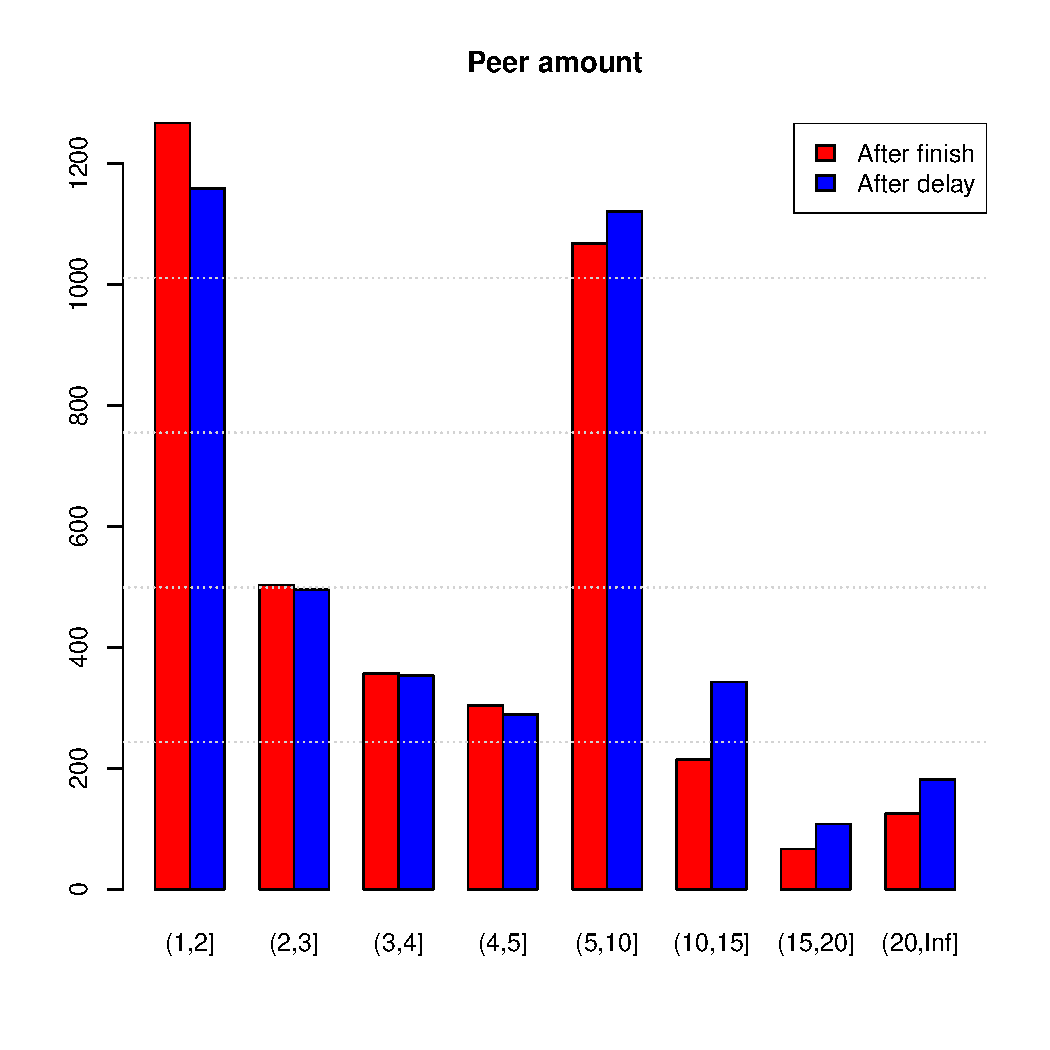
\includegraphics[width=\textwidth]{pics/results/ppredown_t60i30.pdf}
		\caption{Amount of peer discovered}
		\label{fig:peeramount}
	\end{subfigure}
	\caption{Predownload results targeting rarest piece selection.\todo[inline]{create x-y-labels in figure above. Change to use ggplot2}
		}
	\end{adjustwidth}
\end{figure}

Out of 13956 observed swarms, one-third are finished. The rest are failed because of various reasons that will be explained below. The system unable to completely download 4 pieces within time period from 19\% of the swarms. 25\% of the swarm do not have enough piece to mine. Finally, 22\% of the swarm failed to \textit{predownload} under maximum number of attempts. This case can be split into several categories. 

From 3031 swarms that are out of attempts, we could not retrieve any peers information at all from the majority, which contains 2115 swarms (69\%). Another case is when the system could discover the peer, but failed to get piece information from those peers. This case occurred in 175 swarms. From 738 (24\%) swarms, the system could not find any leecher/downloader, thus made it unsuitable for mining. In this case, all observed peers have a complete file. The number of rarest pieces on 3 swarms is less than required piece needed to complete the predownloading. For this particular case, the system already downloaded or has all the rare pieces of this swarm.

On the following experiment we discuss the costs, trade-offs and performance around the observation period of a swarm and the amount of discovered peers. The previous result can be extended in Figure \ref{fig:predownhist} and Figure \ref{fig:peeramount}. Figure \ref{fig:predownhist} shows the distribution of time needed to download 4 of the rarest piece. We only consider successfully downloaded swarm, which totaled 4623 swarms. Most of the swarms can be downloaded in less than 2 minutes. This also includes the time needed to compute which the rarest pieces are. A significant amount of swarms also belong to the 1000-2000 seconds category. Although the time needed to predownload may be increased, we do not recommend to do so. By looking at this figure, the ideal threshold time should be around 30 minute instead of 60 minutes. 


On the right side, Figure \ref{fig:peeramount} shows the increased amount of peer discovered as the result of the enforcement of waiting time. For 10 minutes, we can retrieve more peers information on a swarm. The number of peers for 846 swarms (18\%) has increased with 6112 new peers. The total peers discovered for all the peers before waiting time is 26317, while for after is 32429 peers.

\subsection{Other piece selection}
Based on the result above, finding rare pieces in a swarm is relatively difficult task. In this section, we changed the way the system look for pieces in predownloading for comparison. Instead of looking for the rarest one, we implemented two approaches : sequential and random. In sequential mode, the system will download first 4 pieces. As for random mode, it will look for 4 piece randomly. On contrast with finding the rarest one, these two approaches will immediately decide which pieces they intend to download after first piece has been downloaded. The result can be seen in Figure \ref{fig:predownpseq} and \ref{fig:predownprandom} for sequential mode and random mode, respectively. 

\begin{figure}[h!]
%	\begin{adjustwidth}{-1.5cm}{}
		\begin{subfigure}[t]{0.5\textwidth}
			\centering
			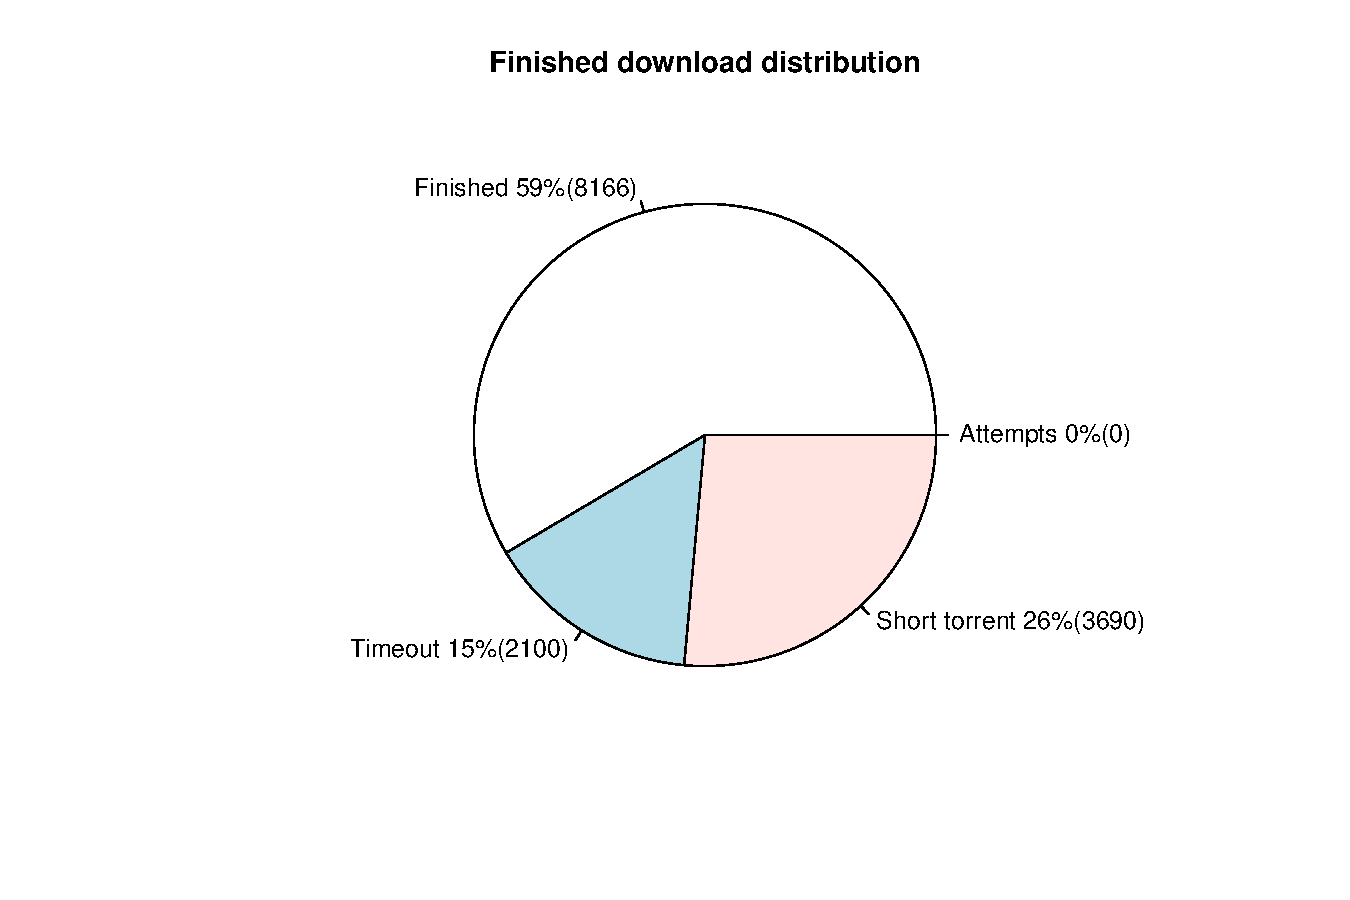
\includegraphics[width=\textwidth]{pics/results/dpredown_sequential.pdf}
			\caption{Success percentage in sequential piece selection}
			\label{fig:predownpseq}
		\end{subfigure}
		~
		\begin{subfigure}[t]{0.5\textwidth}
			\centering
			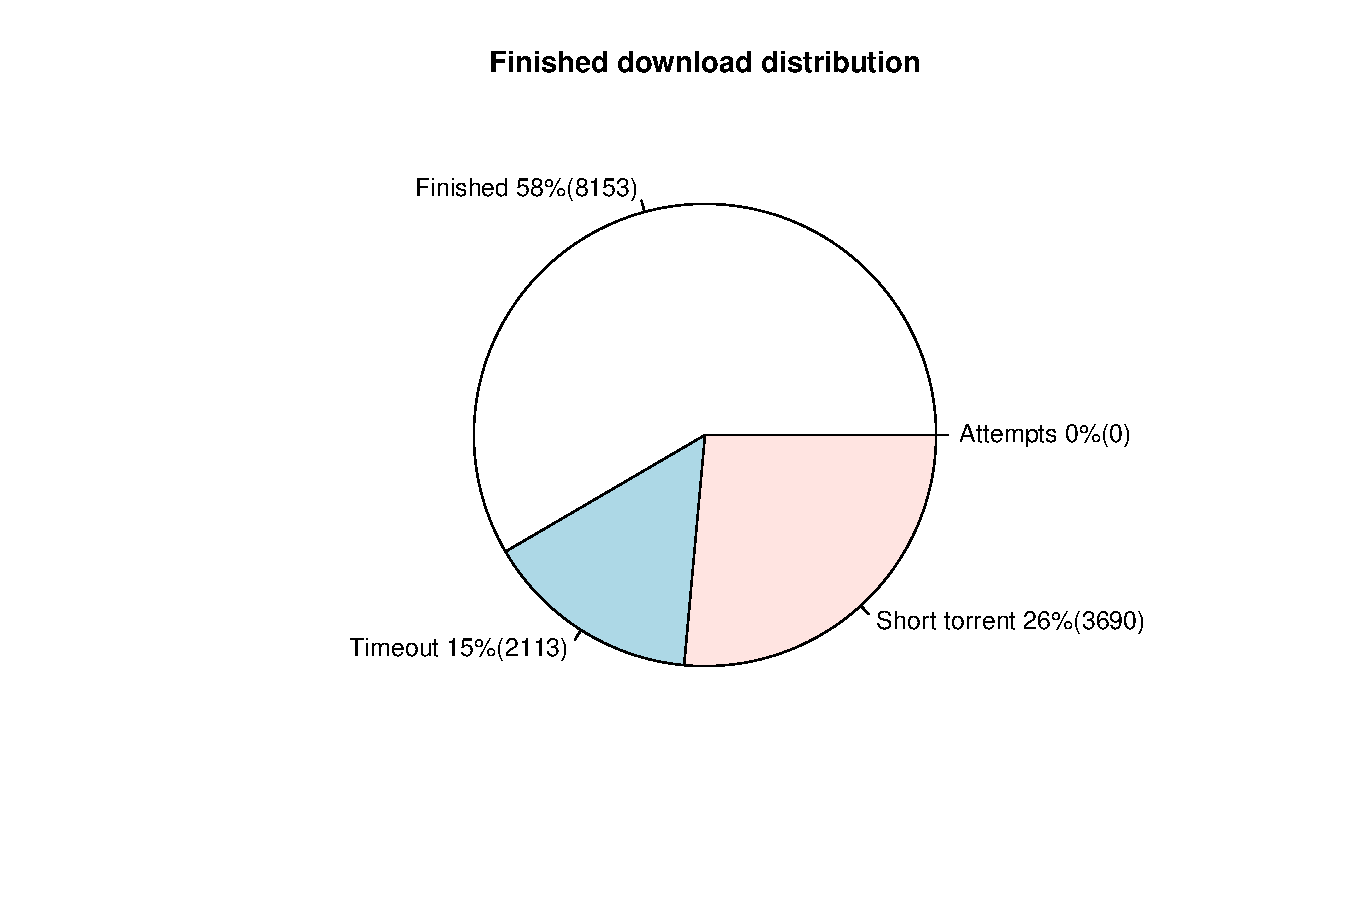
\includegraphics[width=\textwidth]{pics/results/dpredown_random.pdf}
			\caption{Success percentage in random piece selection}
			\label{fig:predownprandom}
		\end{subfigure}
		\caption{Predownload success percentage for other piece selection approach.}
%	\end{adjustwidth}
\end{figure}

From the Figure \ref{fig:predownpseq} and \ref{fig:predownprandom}, it clearly shows that the number of swarm that successfully downloaded in both sequential and random method has increase significantly compared to initial method. The number of timeout swarm also reduced by a few. Both approaches resulting 0 for attempted failure swarm. This clarify that most of the swarms in this experiment are active. However, some of them do not have any leecher/downloader at the time of experiment. One that distinguish these alternative method from initial method is that these do not need to collect both peer and swarm information extensively. 

Based on the results above, it is clear that most of the swarms collected by the crawler is mostly alive. However, some of them do not have any leecher, therefore, render them as inactive. Rarest piece method can filter those unwanted swarm as they are not suitable for mining. This method can cut the number of prospected swarm for mining to one-third of total swarm which is beneficial to reduce the complexity for the next phase. Moreover, its behavior is similar to \textit{share mode} in \textit{libtorrent} by only downloading rarest piece that we will be able to upload in the future.

\section{Choosing the best swarm}
\label{section:chooseswarmexp}
The main element of credit mining is to find and prospect which swarm to mine in order to get high return of investment. We define the return of investment (ROI) with \textit{net upload gain}. In prior work, \citeauthor{2015:creditmining:capota} has introduced three policies to choose a swarm. In this thesis, we introduce \textit{scoring policy} which considers other elements as part of a swarm's worth. The following experiment is specifically designed to be simple and able to validate all core components and algorithms of our credit mining research. All conditions are controlled and do not rely on external elements such as trackers or DHT nodes. Our first validation experiment tests the basic credit mining swarm selection algorithm.

The experiment run for three hours. The number of swarm is this experiment is 10, each has the same file size with various number of seeders and fixed number of 5 downloaders. A single credit miner then starts prospecting these swarms and should select the most underseeded swarm. Each swarm has different peer as publisher as well as dedicated seeders. Each peers only have 1 role, either as a publisher, seeder, or downloader. The credit mining system actively choose at most 3 of those swarm to mine at a time. We set share mode target as 2 instead of the recommended 3 because this experiment only has few peers for each swarm. The complete scenario and settings for this experiment presented in the appendix. In this experiment, we use \textit{peer translation} function to interpret the number of seeder and leecher in a swarm.

By its nature, credit mining system only able to control what swarm to choose and how long the mining in one session is. After a swarm has been chosen, \textit{libtorrent} with its \textit{share mode} will do the rest. This causes a slightly different results in each experiment. However, if the swarm selection constantly choose a particular swarm, we expect the trend to be similar. 

\subsection{What the policies choose}
\begin{figure}[h]
	\centering
	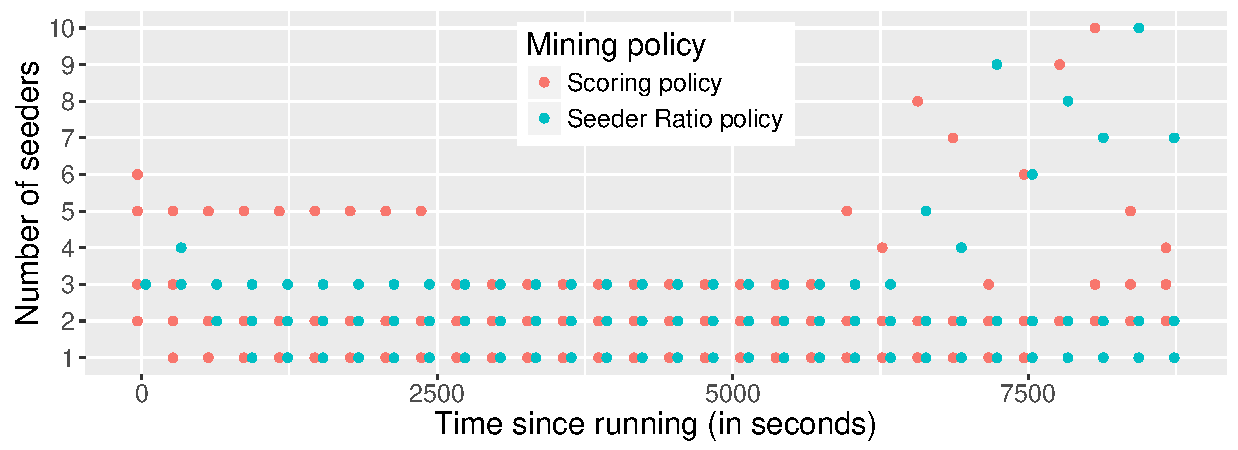
\includegraphics[width=\textwidth]{pics/results/scsr_notrig_scatter.pdf}
	\caption{Seeder ratio and scoring policy swarm selection.}
	\label{fig:scatterscsrnotrig}
\end{figure}

Figure \ref{fig:scatterscsrnotrig} shows how the policy chooses swarm from time to time. At the beginning, we do not have many information of the swarms yet. This causes peer translation function is less accurate than it should be. But as the time goes on, more information can be collected, swarm information is stabilized, and both policy and peer translation function become more accurate. Near the end of the experiment, the effect is inverted. We got complete information on mined swarms, but not for the others. As soon as the system saw that the swarm has sufficient number of seeder, it will switch to other swarm. However, the system still sees other swarm with obsolete information. Both of the policies have to rejoin other swarm to know its updated information. That explains the policy choice dispersion in the last 40 minute near the end.
% In this specific case, \textit{scoring} policy perform better by faster to stabilize the next swarm to mine. It can be seen from the last two observation that it already choose the next undersupplied swarm. 

In this experiment, it shows that both seeder and scoring policy have similar choice of the swarms. That is because scoring policy was built on top of seeder policy. The feature that distinguish one swarm from another on this experiment is only the number of seeder and leecher. Because of that, scoring policy will have similar performance compared to seeder policy. 

\subsection{Obtained gain by the selection}
The next experiment is conducted to know the actual gain obtained as a result of swarm selection presented in Figure \ref{fig:scatterscsrnotrig}. 

We shows the obtained gain of applying seeder ratio policy in Figure \ref{fig:simplesrnotrig}. A swarm with 2 seeders is dominating the result. The rest of the selected swarm is relatively constant most of time. Swarm \texttt{1gb\_2} average seeding speed is 61 kB/s, which is more than half of the maximum speed on a single peer. This swarm also used significant resource, which more than 80\% of the maximum upload rate, for 44.67\% of its lifetime. 

In Figure \ref{fig:simplescsrnotrig}, scoring policy is applied. Unsurprisingly, the trend is similar. This time, the gain is much higher, almost twice as of the seeder policy. The dominating swarm is exactly the same, which is \texttt{1gb\_2}. Average upload speed for this swarm is 94.4 kB/s with 90\% of the observation is taking more than 80\% of the maximum upload rate. It is clear that the factor that limits credit mining system obtained higher gain is the maximum upload rate. 

\begin{figure}[h!]
	\begin{adjustwidth}{-2.5cm}{}
		\begin{subfigure}[t]{0.7\textwidth}
			\centering
			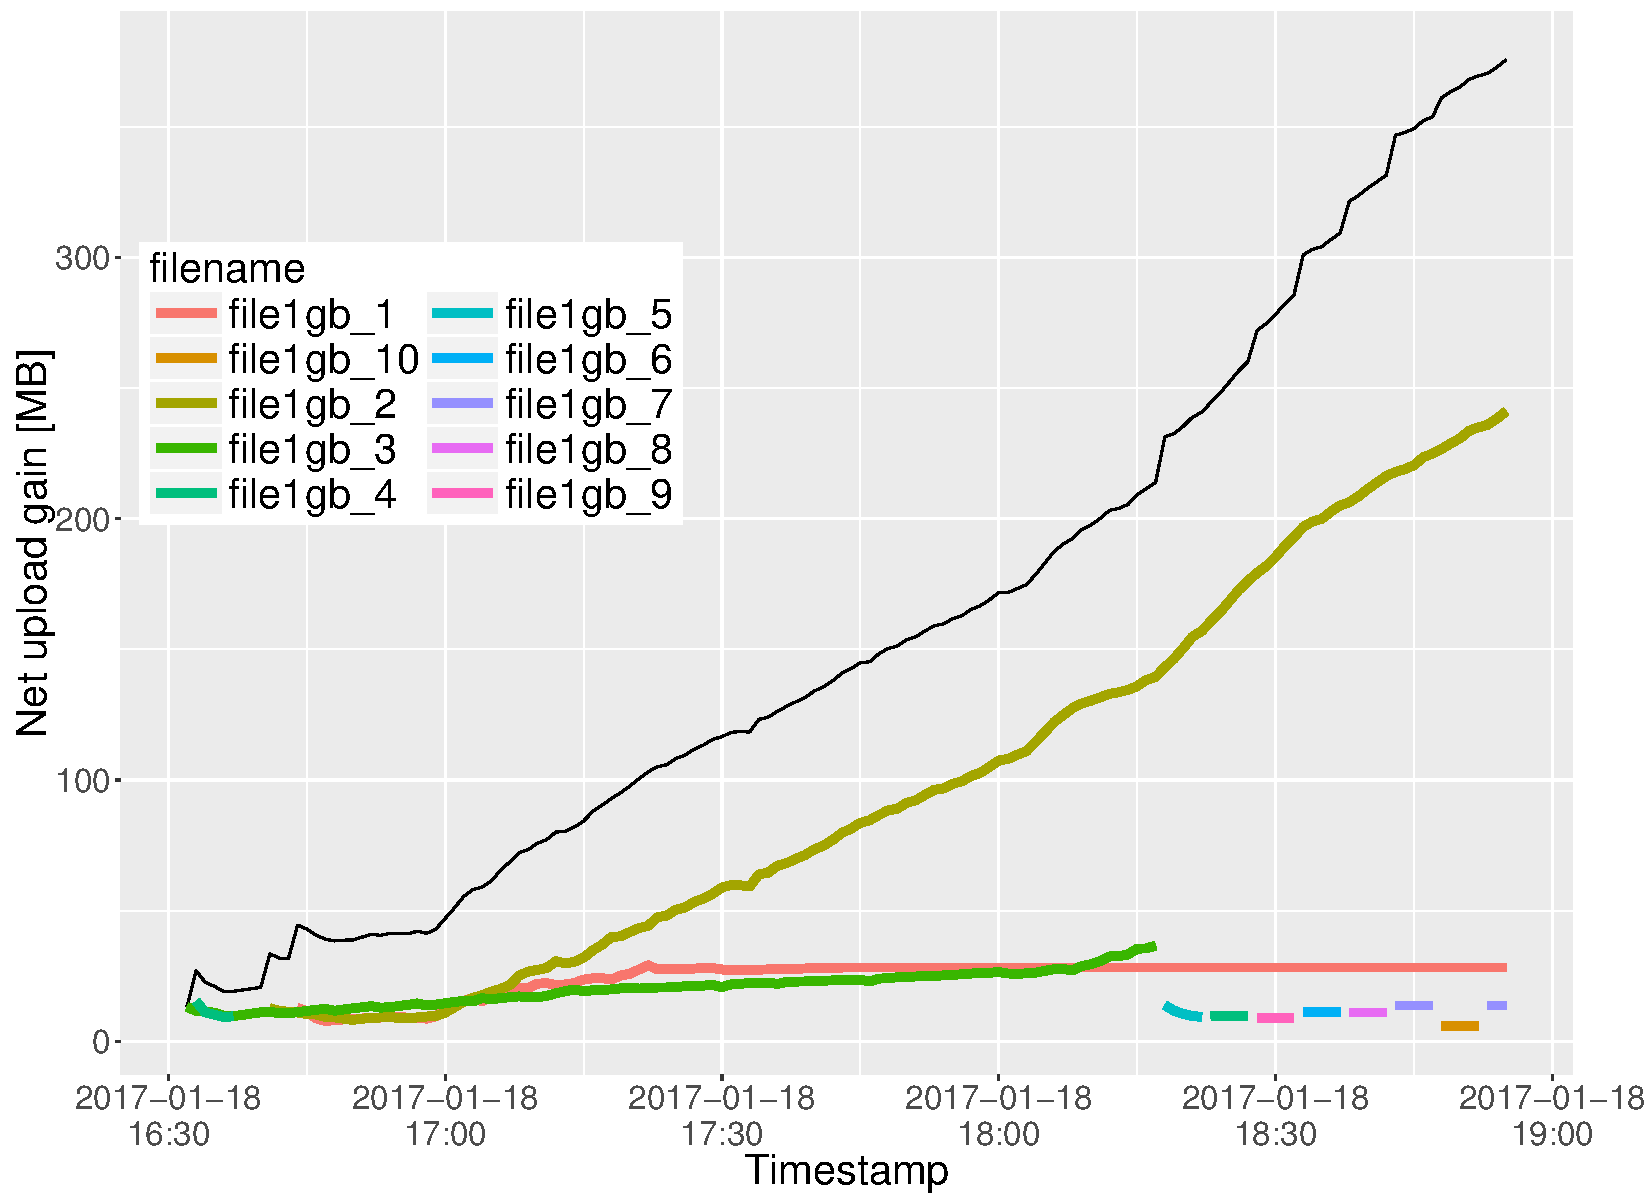
\includegraphics[width=\textwidth]{pics/results/simple1_sr_notrig.pdf}
			\caption{Seeder ratio policy gain.}
			\label{fig:simplesrnotrig}
		\end{subfigure}
		~
		\begin{subfigure}[t]{0.7\textwidth}
			\centering
			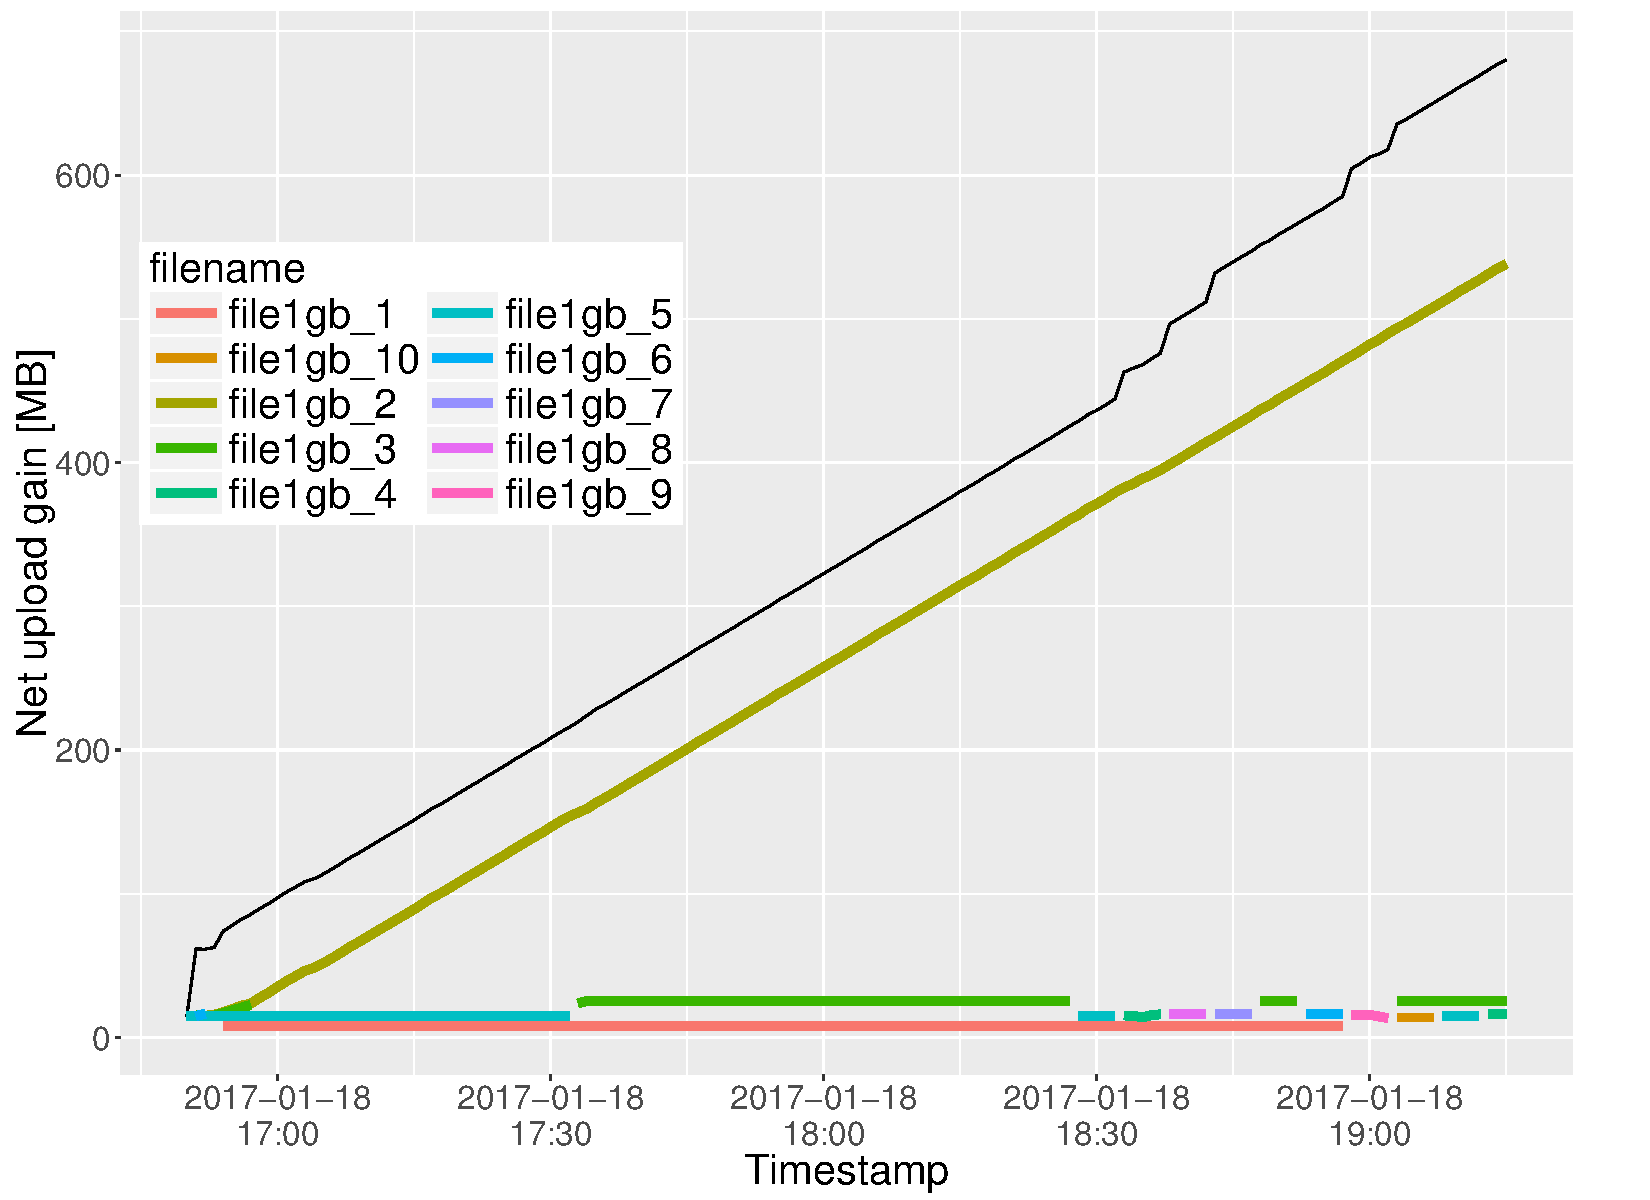
\includegraphics[width=\textwidth]{pics/results/simple1_scsr_notrig.pdf}
			\caption{Scoring policy gain.}
			\label{fig:simplescsrnotrig}
		\end{subfigure}
		\caption{Net upload gain of both policies.}
	\end{adjustwidth}
\end{figure}

After we observed two results, we come with two conclusions. First, our hypothesis about the similar choice in this particular experiment with on of the policies is stand corrected. Although the gain is significantly different, it was not directly caused by the mining system. Instead, it is part of the \bt~protocol that build up the download and upload speed. Second, although the resource may be used to its full capacity like shown in Figure \ref{fig:simplescsrnotrig}, it is entirely possible that it is not used efficiently. This is shown by the inactivity from the other swarms. Net upload gain for other swarms are barely increasing for both cases. 

After analyzing the result, we find out that the root cause of swarm inactivity caused by \textit{libtorrent}'s \textit{share mode} algorithm. The condition to download more pieces is too strict. In static environment such as this experiment where there are no new peers in the long term, share mode will perform relatively poor as hinted by our argument in section \ref{section:sharemode}. Therefore, the seize up condition on the swarm occurred. In this state, the only possible solution is to upload the pieces the miners have. In saturated and static environment, this can only be solved by adding new peers. 

\subsection{The effect of inciting swarms}
As soon as we realize that there is a possible swarm bottleneck case in \textit{libtorrent}'s \textit{share mode}, we came up with this idea. Its purpose is to avoid swarm inactivity and to stir whenever the swarm suffers from bottleneck. This was implemented on lower level of the selection policy, so it will not change how the credit mining system select a swarm. The swarm selection result of both seeder ratio and scoring policy with incitement enabled is shown in Figure \ref{fig:scatterscsrtrig}.

\begin{figure}[h]
	\centering
	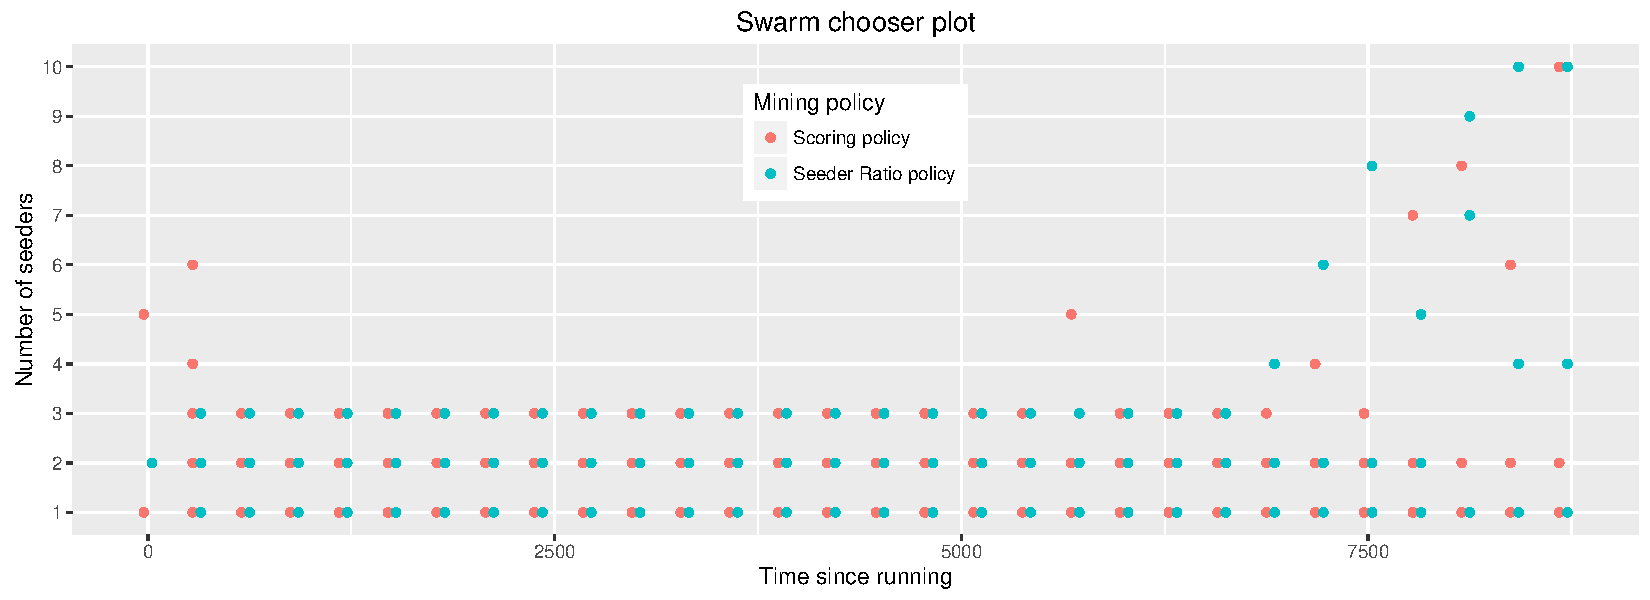
\includegraphics[width=\textwidth]{pics/results/scsr_trig_scatter.pdf}
	\caption{Seeder ratio and scoring policy swarm selection with incitement enabled.}
	\label{fig:scatterscsrtrig}
\end{figure}

\begin{figure}[h!]
	\begin{adjustwidth}{-2.5cm}{}
		\begin{subfigure}[t]{0.7\textwidth}
			\centering
			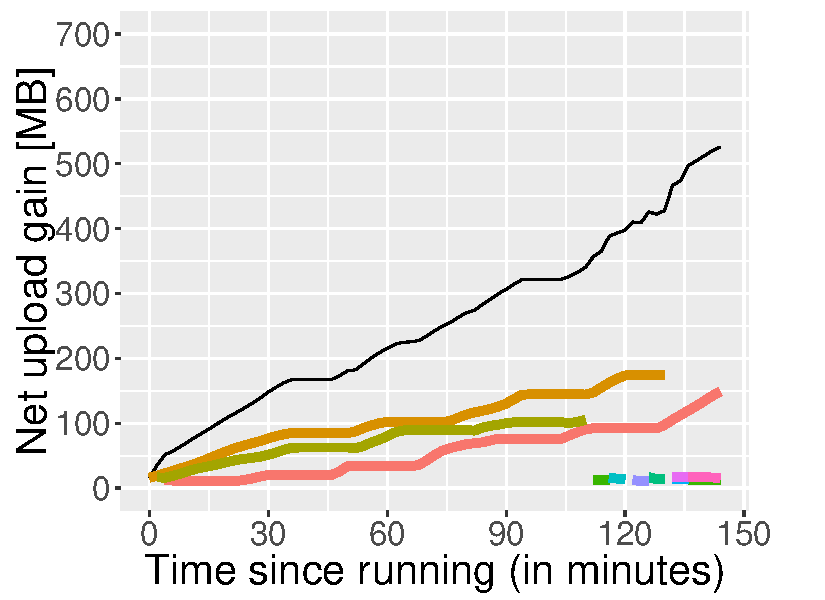
\includegraphics[width=\textwidth]{pics/results/simple3_sr_trig.pdf}
			\caption{Seeder ratio policy gain with incitement enabled.}
			\label{fig:simplesrtrig}
		\end{subfigure}
		~
		\begin{subfigure}[t]{0.7\textwidth}
			\centering
			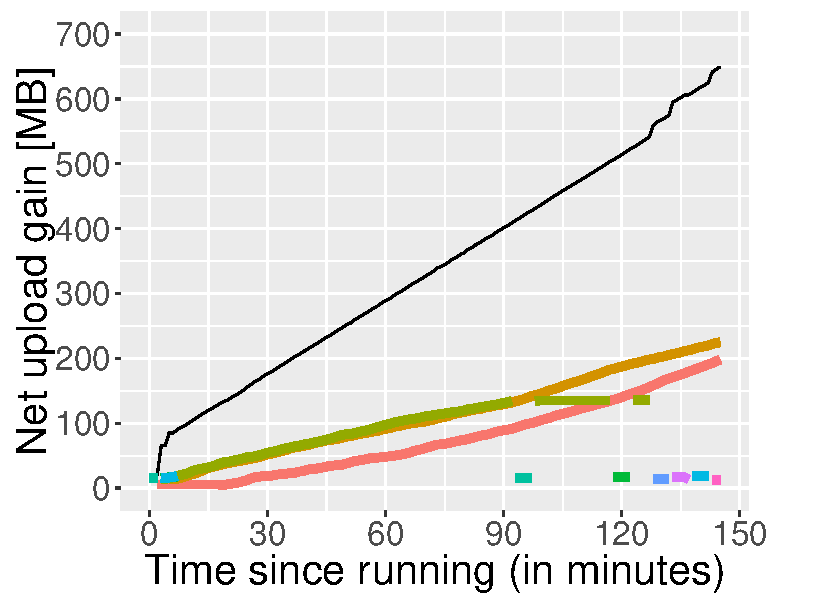
\includegraphics[width=\textwidth]{pics/results/simple1_scsr_trig.pdf}
			\caption{Scoring policy gain with inciting and enforcing blacklisting.}
			\label{fig:simplescsrtrig}
		\end{subfigure}
		\caption{Net upload gain of both policies with incitement enabled.}
	\end{adjustwidth}
\end{figure}

With incitement enabled, inactive swarms tend to gain more credits when mined. Figure \ref{fig:simplesrtrig} shows the case for seeder ratio policy. Compared to previous results, this has significant increase of net upload gain. From the figure, we can see that there are many bumps that lead to the increasing amount of gain. Total piece incited by each swarm is 20, 12, and 12 for \texttt{1gb\_1}, \texttt{1gb\_2}, and \texttt{1gb\_3}, respectively. As each of the incitement need 4 piece to download, the number of incitement matches with the bumps in the Figure \ref{fig:simplesrtrig}. 

On the contrary, in scoring policy, the effect of incitement is not significant. It shows on Figure \ref{fig:simplescsrtrig}. There are only two incitement, one for \texttt{1gb\_1} and the other for \texttt{1gb\_3}. Only incitement for \texttt{1gb\_1} can be seen in the figure. On the other hand, when incitement of swarm \texttt{1gb\_3} was executed, the miner coincidentally decide to switch for another swarm in the next turn. This swarm then will be stopped. Therefore, the improvement of the gain is not visible. Albeit the less impressive performance, the total gain obtained similar to the near-full capacity as shown in Figure \ref{fig:simplescsrnotrig}.

% 100 swarm for 12, 24. 500 swarm for 24h
\section{Comparing obtained gain with prior work}
In this experiment, we will evaluate the result of the proposed method compared to prior work. The comparison experiment will be run 24 hours. As a note, prior work run its experiment for 2 days (48 hours) straight. Etree.org will be used as mining source because other sources are not compatible with the prior work. It is also not compatible with our experiment framework, gumby, to test in closed environment. The recommended parameter on prior work is by setting credit mining system with SeederRatio policy, target ratio 3, and 5 minute swarm interval although in their argument, setting target ratio as 1 gives higher net upload gain. In our experiment, we will use the same parameter and configuration. The result will be shown in Figure \ref{fig:oldetree24}.

For the proposed method, we applied scoring policy with incitement enabled. Other parameter will be kept the same with previous experiment. The result of this experiment will be compared to the one that run on top of the prior work. The result of obtained gain will be presented in Figure \ref{fig:newetree24}. Note that the axis that represents net upload gain is logarithmic.

\begin{figure}[h]
	\begin{adjustwidth}{-2cm}{}
		\begin{subfigure}[t]{0.6\textwidth}
			\centering
			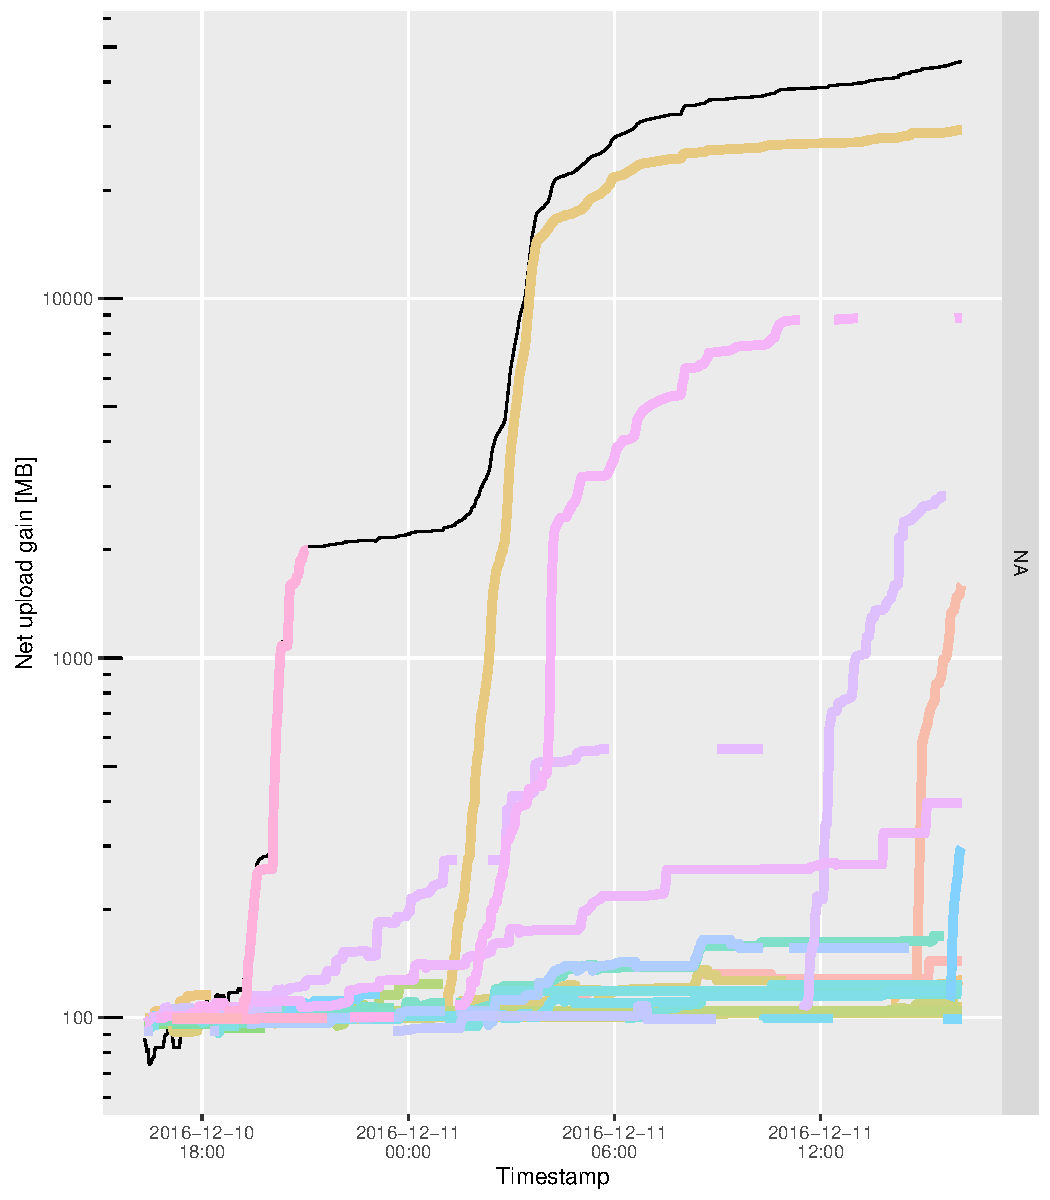
\includegraphics[width=\textwidth]{pics/results/b136.pdf}
			\caption{24 hour new experiment.}
			\label{fig:newetree24}
		\end{subfigure}
		~
		\begin{subfigure}[t]{0.6\textwidth}
			\centering
			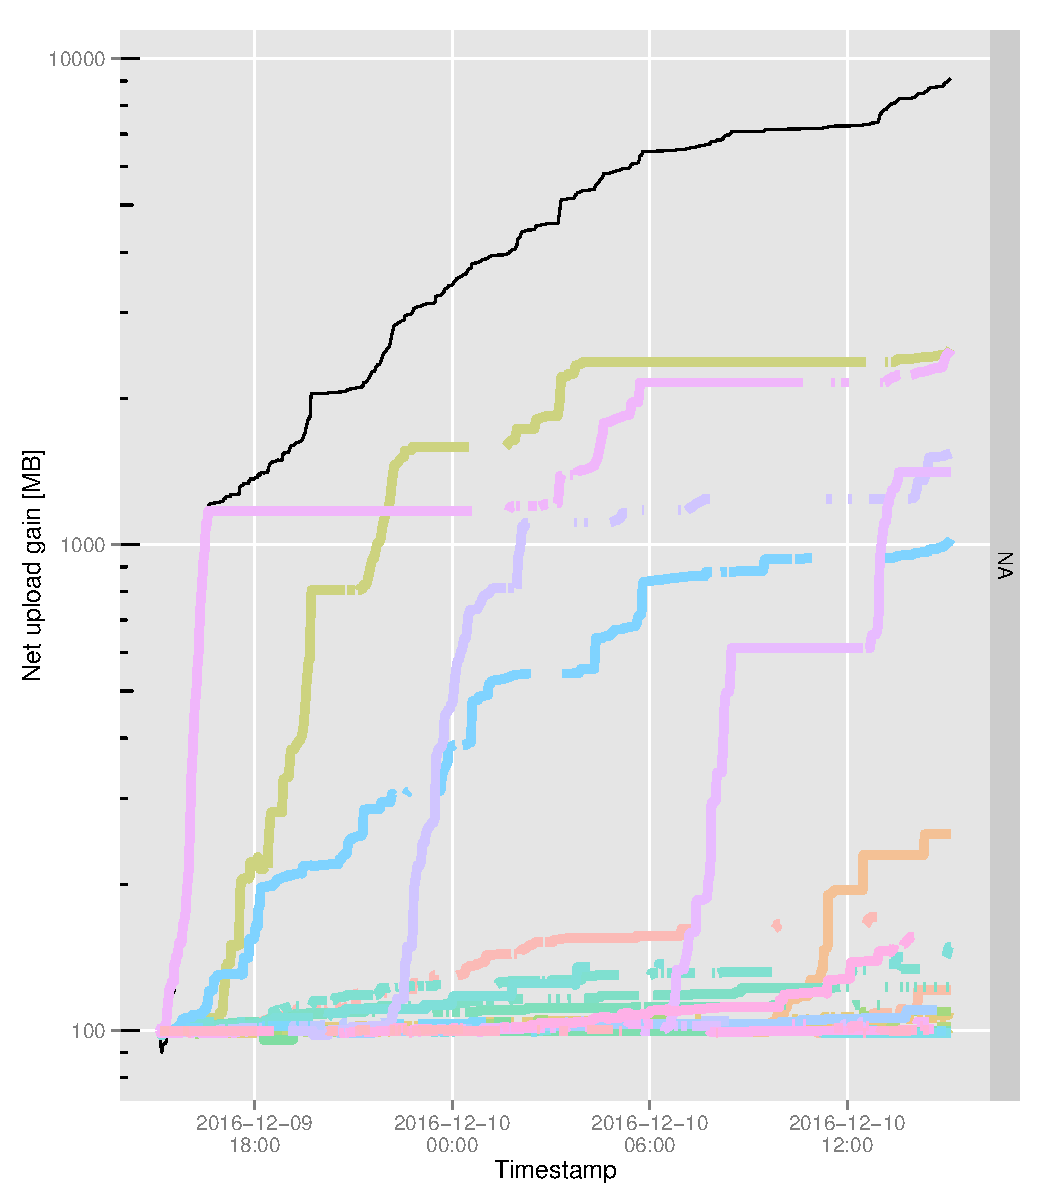
\includegraphics[width=\textwidth]{pics/results/m138.pdf}
			\caption{24 hour old experiment}
			\label{fig:oldetree24}
		\end{subfigure}
		\caption{New vs old experiments (run separately) result on 24 hour (\textit{seederratio} policy)}
	\end{adjustwidth}
\end{figure}

From the figures presented, we can find one similarity. Both of the system dominated only by a few swarms. It means that not all the recent swarms is popular. Popular swarm means more leecher which impact the overall credit gain. \todo{re-run with updated code} For the main difference, we found two aspects that shows new credit mining system is better : policy stability and reducing idleness. In new system, thanks to scoring policy, the miners do not need to unnecessarily switches swarm. It shows that the lines tend to more continuous compared to one in prior work. When the line is not in sight, it means that particular swarm was not selected in this round. It will be shown in the next experiment that this aspect also will be indirectly reflected in swarm overall stability.\todo{maybe need to compare the policy head-to-head}. Second aspect is the idleness of a swarm. It represented in straight horizontal line in the figures. We can successfully reduce the idle swarm by enabling incitement. In this experiment, when net upload gained is more than 500 MB, none of the swarm is idle. On the contrary, some swarms in prior work are idle, even when the gain already high. We aware in the lower section, some swarms in new experiment are idle. This is because the minimum gain needed for the incitement to be able to work could not be reached.

\section{Swarm performance with credit mining}
%\todo[inline]{WORK ON PROGRESS - Waiting for results}
%\todo[inline]{single swarm}
%\todo[inline]{scoring inside}
%\todo[inline]{average net upload gain on involved miners}

After we confidently get high return gain from the previous results, it is worth to find out what effects credit mining has to the community. The experiment run in the same setting as from Section \ref{section:chooseswarmexp}, except we add more miners instead of one. We also use scoring policy as default and enable both predownload and incitement execution. Other parameters are left default.

Figure \ref{fig:swarmnocmperf} shows the average download speed of all the member in each of the swarm. In this experiment, no credit mining system are active. Because the experiment was static, the speed is constantly stable. As expected, the more a swarm has seeder, the higher download speed will be reached for all other peers in that swarm. Some of the swarms has reached its maximum download speed such as \texttt{1gb\_8}, \texttt{1gb\_9}, and \texttt{1gb\_10}. We will take this result as base figure for the next experiment.

\begin{figure}[h]
	\centering
	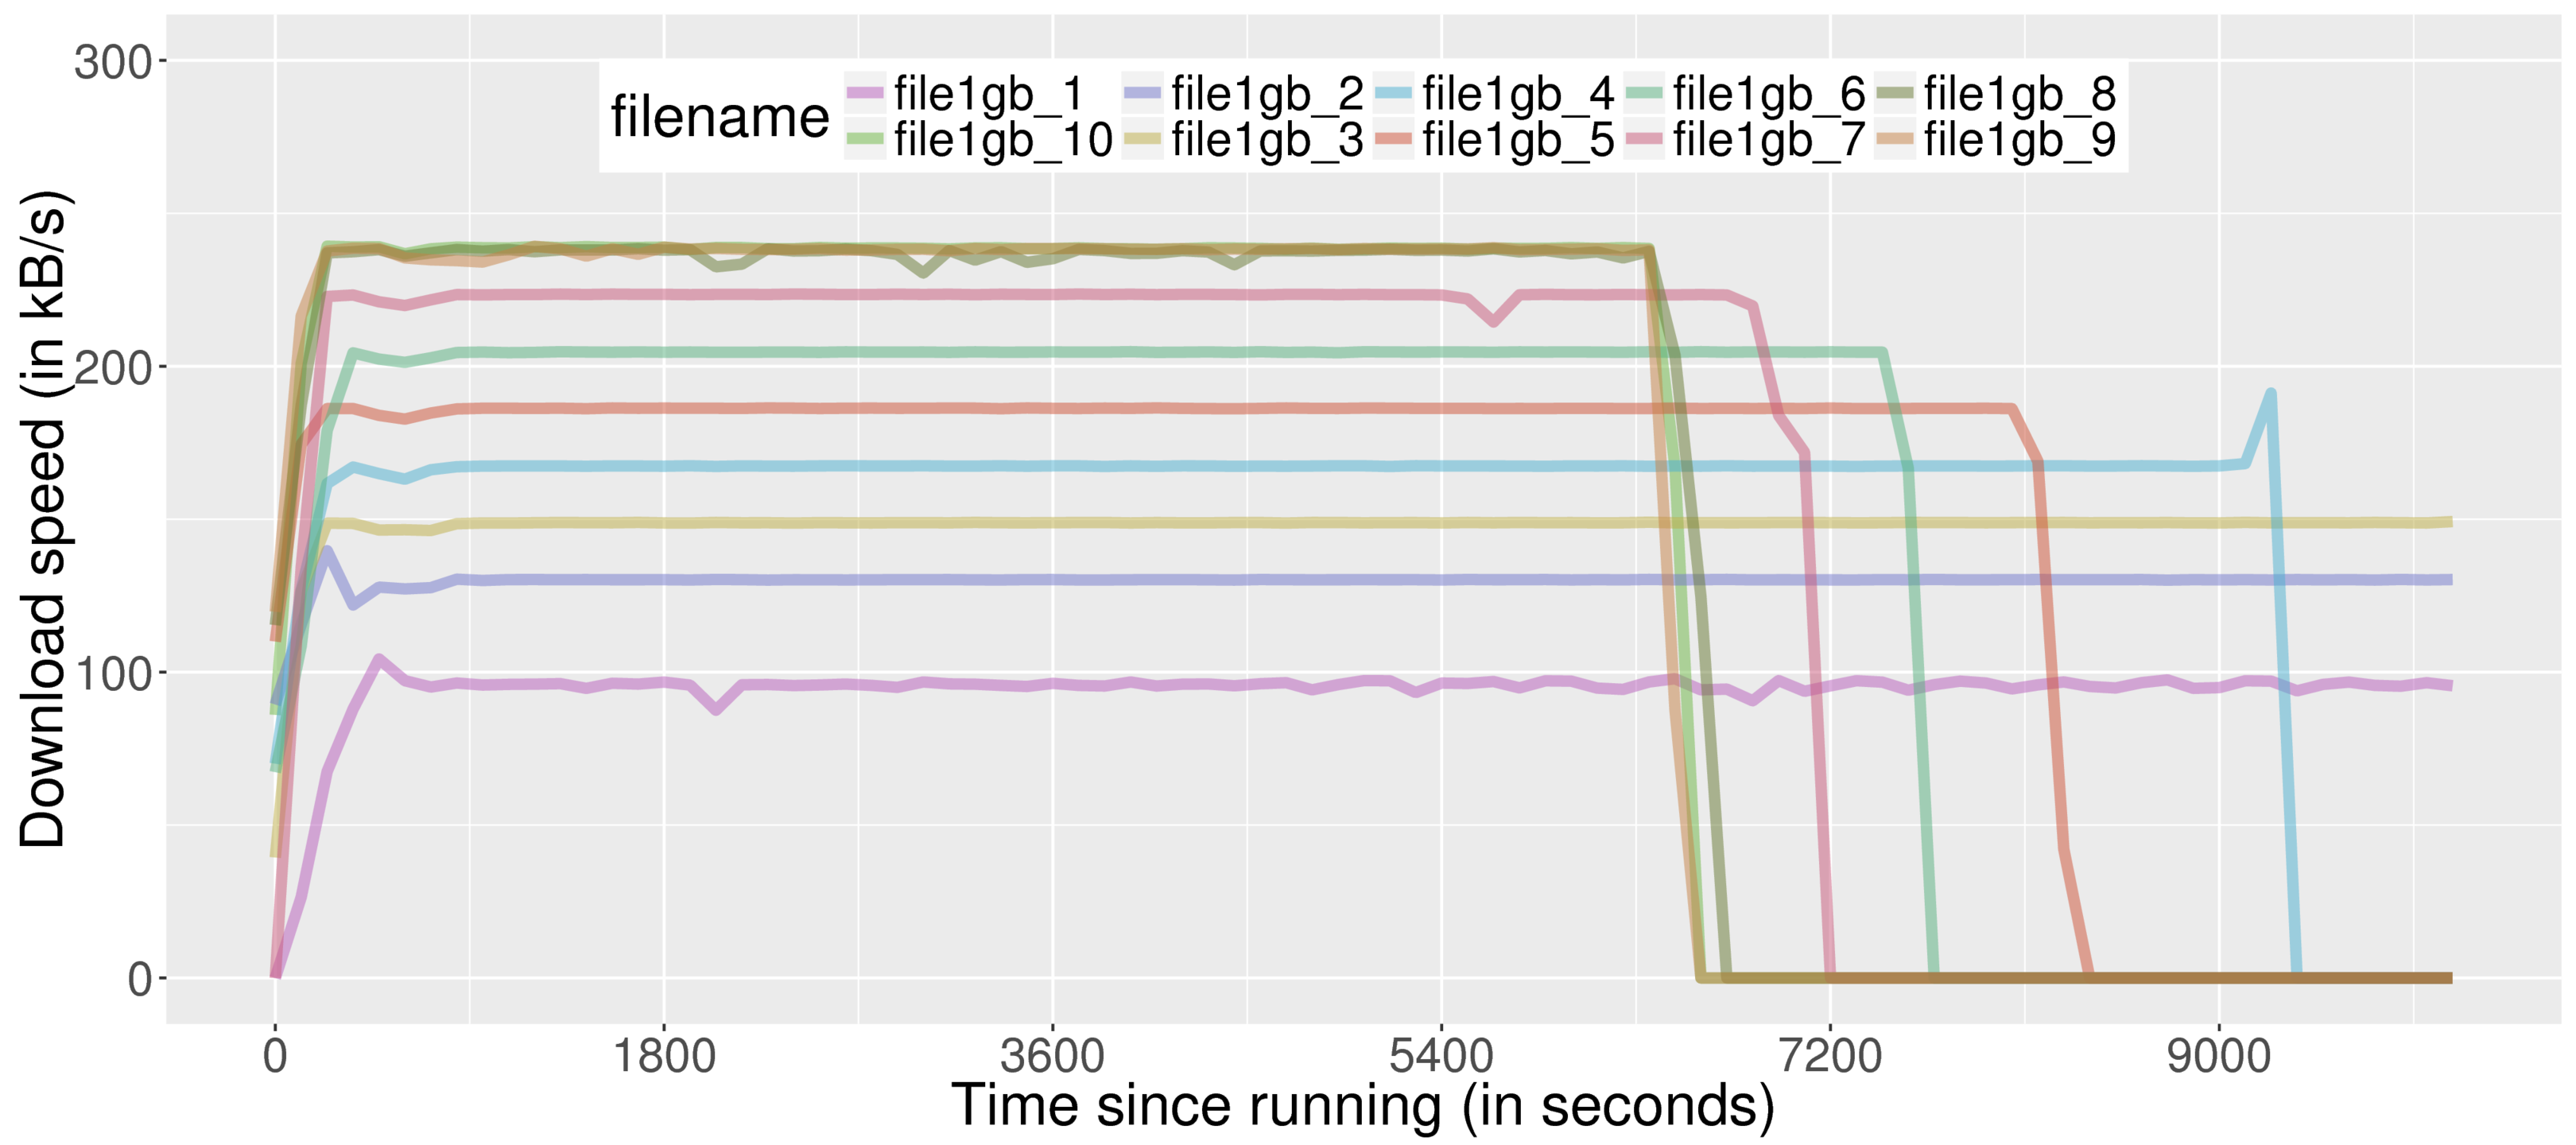
\includegraphics[width=\textwidth]{pics/results/swperf_n2.png}
	\caption{Swarm performance without credit mining}
	\label{fig:swarmnocmperf}
\end{figure}

Next, we will introduce credit mining system in the swarms. We start by spawning credit mining system as much as the number of downloader, which is 50 node. Those are dedicated miners and all of those started simultaneously. Figure \ref{fig:swarmcmperf} shows the average download speed from all the downloaders for each of the swarm.\todo{add more statistical data here} 

There are two noticeable drawbacks when introducing credit mining system to the swarm : (i) the downloaders download speed become unstable, and (ii) the download speed of one swarm might indirectly affect other swarm. First drawback is exist because the miners might not have complete information of all the swarm at the same time. Moreover, a miner also seen as leecher from another miner's perspective. Currently there are not any mechanism to distinguish the miners and to let them communicate each other. On top of that, the nature of the credit mining system is to switch swarm source periodically. Combining these two factors, that explains the unstable download speed although it is generally higher than the base experiment. Second drawback is caused by the credit mining behaviour that unevenly distribute the bandwidth among all the swarms. The increasing download speed in a swarm may cause decreasing speed on another swarm. When a miner switches swarm to join another swarm, it will left the old swarm with lower piece availability because miners tend to only have rarest pieces. Then at the next round, new miners (if necessary), join this swarm. In this stage, new miners have obsolete information on the swarm, including the piece availability and its distribution. It will then download the rarest piece again from seeders, thus temporarily reduce download speed of the downloader. \todo{rephrase, convoluted} Note that this case is not always happen. The miner may not need to redownload rarest piece. Moreover, stayed miner has higher chance to increase its upload gain even more because miner that has similar rarest pieces has left the swarm. This also explain the case where the download speed is not decreasing.

\begin{figure}[h!]
	\centering
	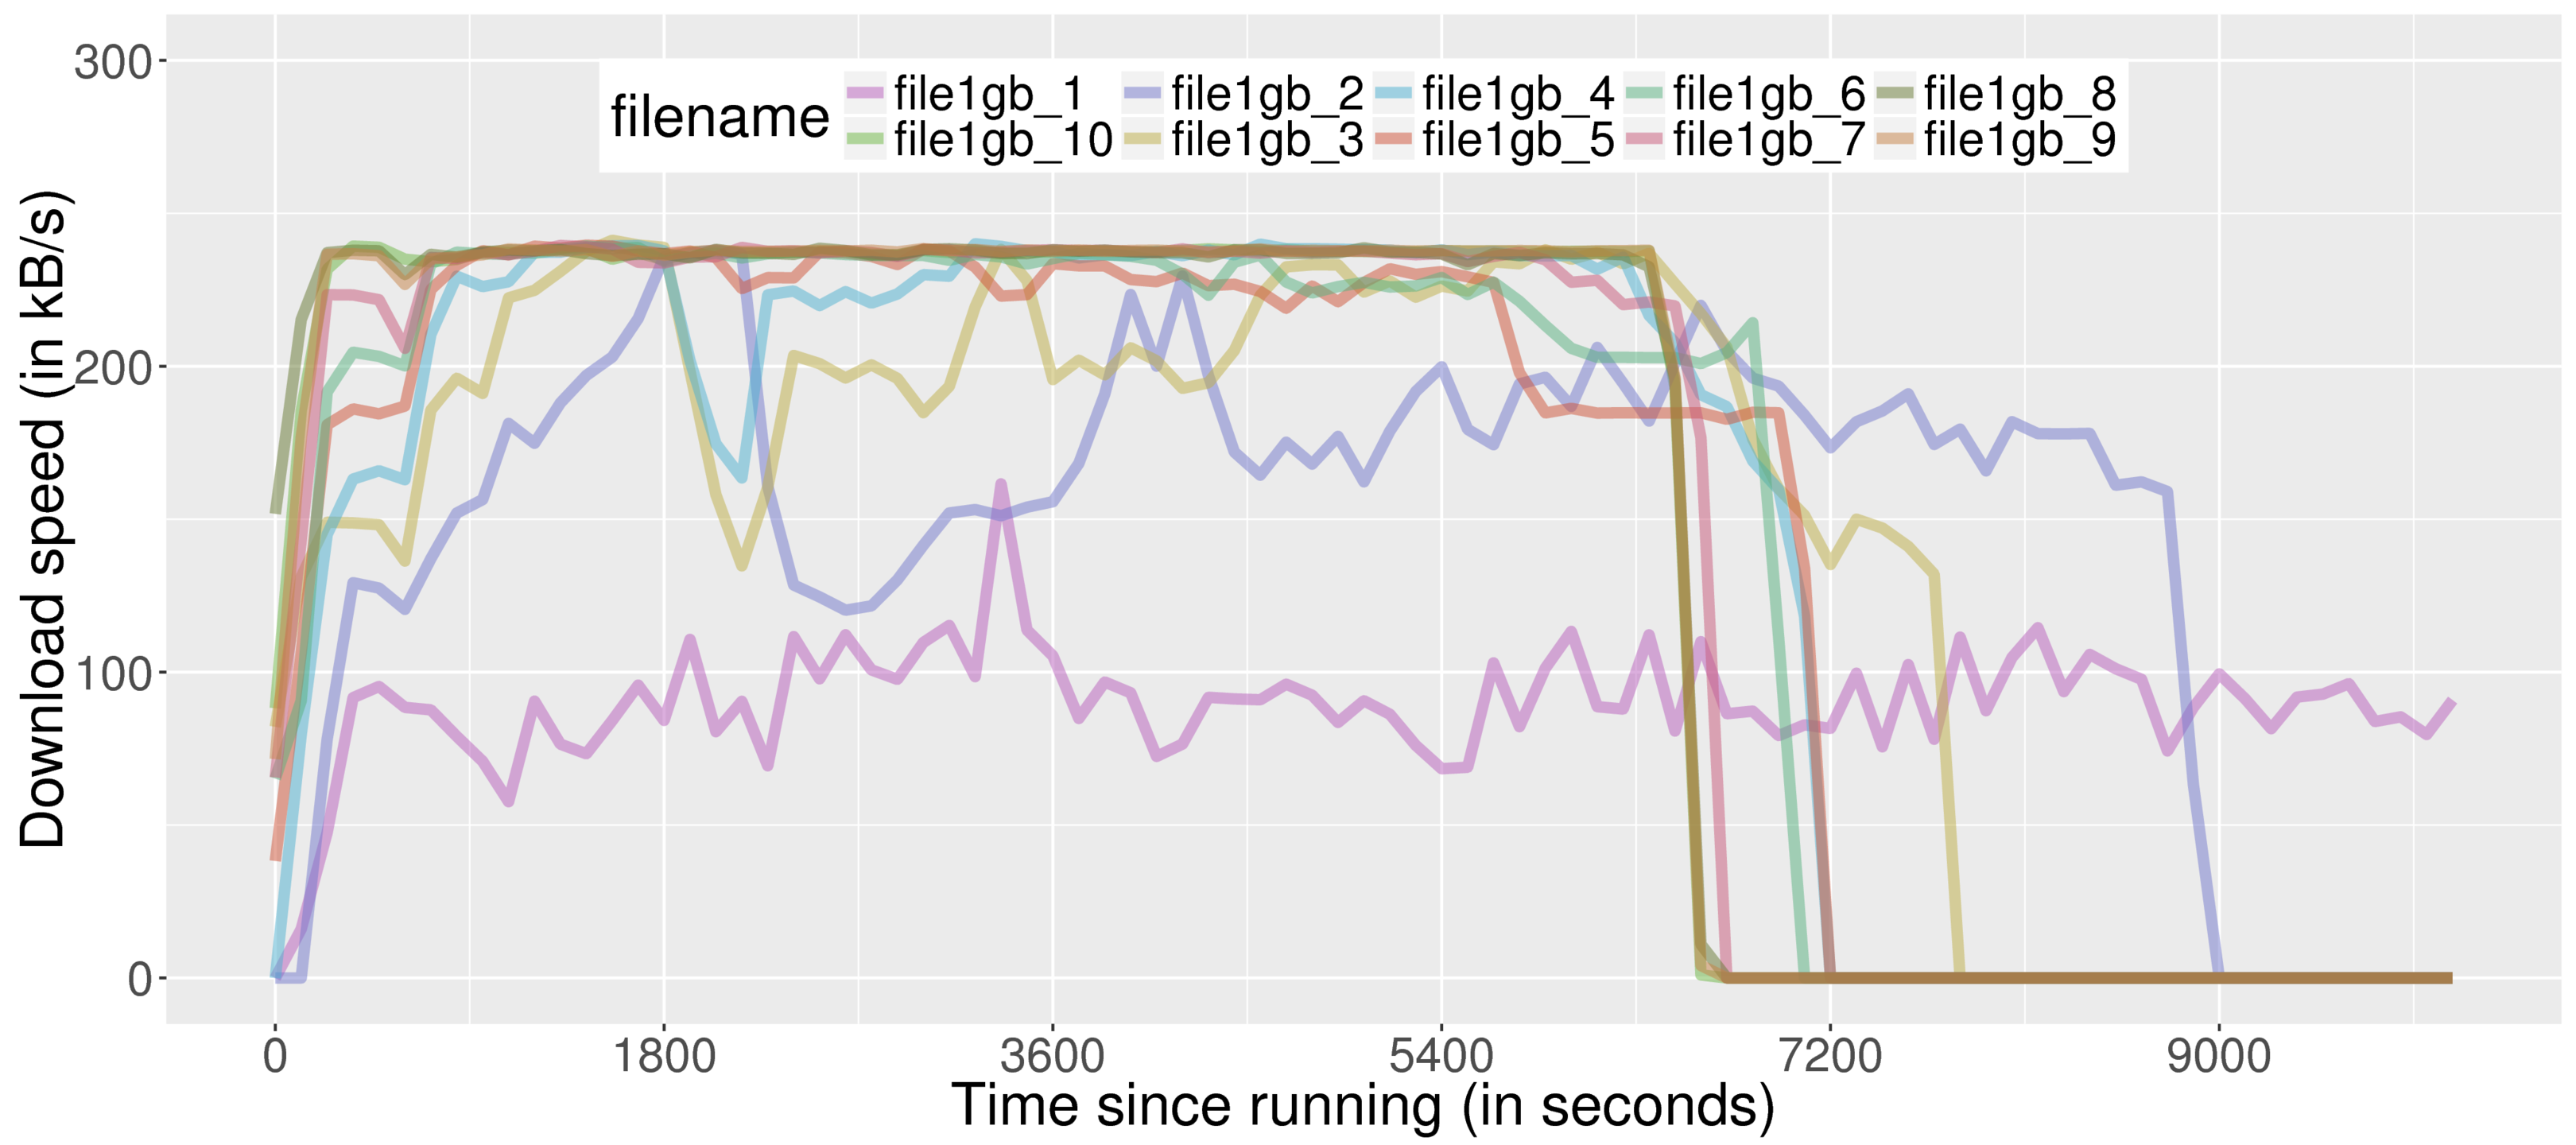
\includegraphics[width=\textwidth]{pics/results/swperf_sc2.png}
	\caption{Swarm performance with credit mining in the swarm (50 peers)}
	\label{fig:swarmcmperf}
\end{figure}

\subsection{Parameters variation and its effect on swarms}

Figure \ref{fig:swarmcm25perf} : 25 miner instead of 50. Slower.

\begin{figure}[h!]
	\centering
	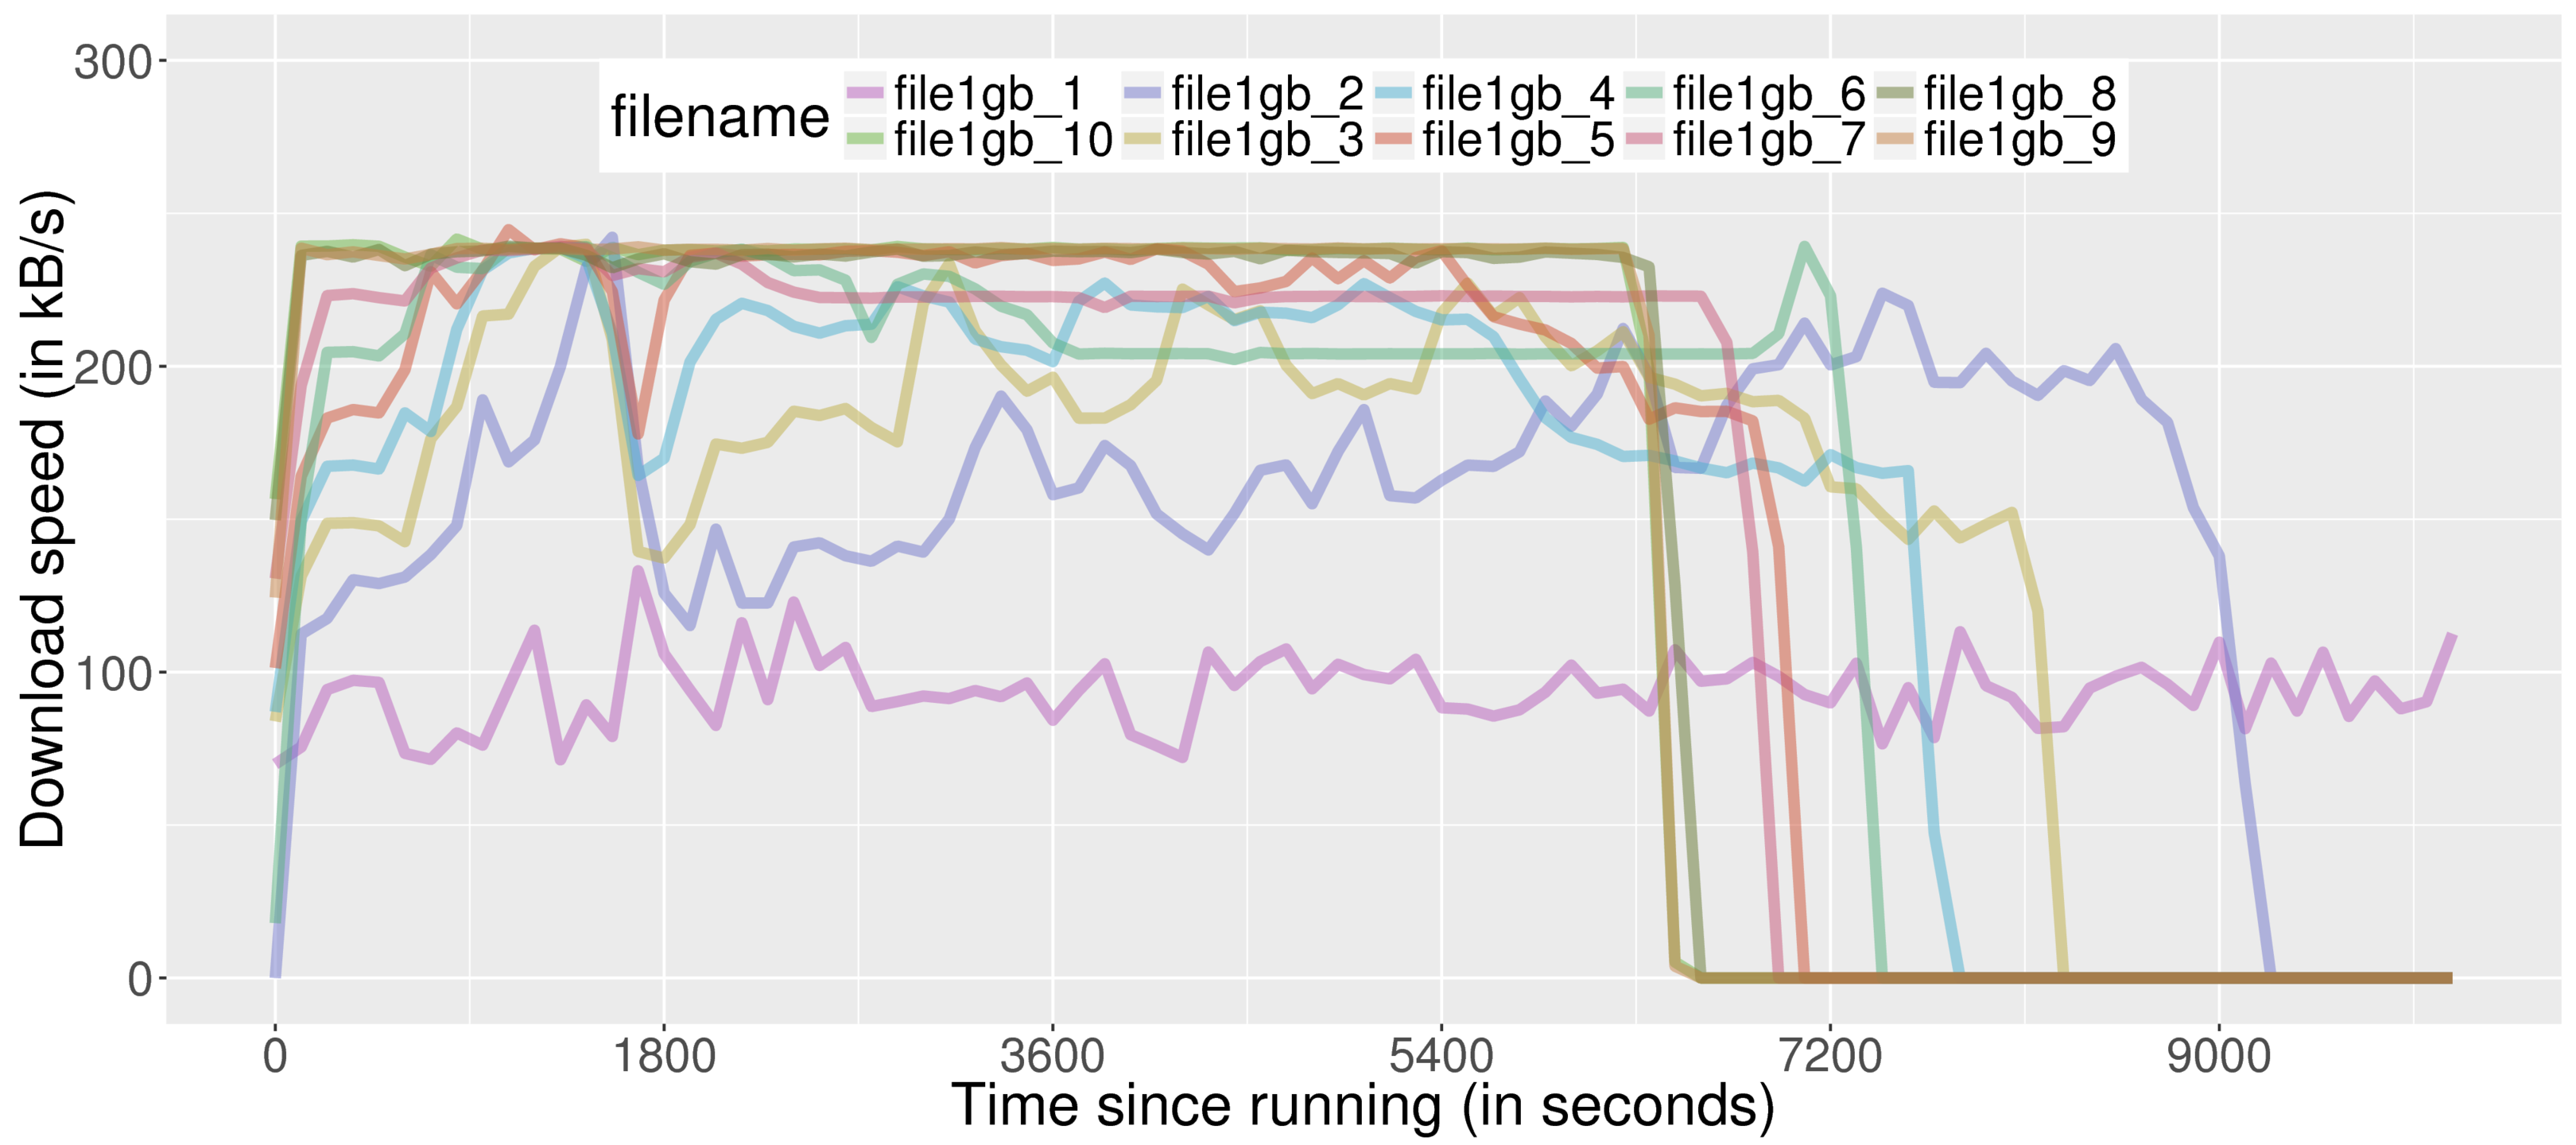
\includegraphics[width=\textwidth]{pics/results/swperf_sc2_25.png}
	\caption{Swarm performance with credit mining in the swarm (25 peers)}
	\label{fig:swarmcm25perf}
\end{figure}

Figure \ref{fig:swarmcm10perf} : 10 miner instead of 50. Slower.

\begin{figure}[h!]
	\centering
	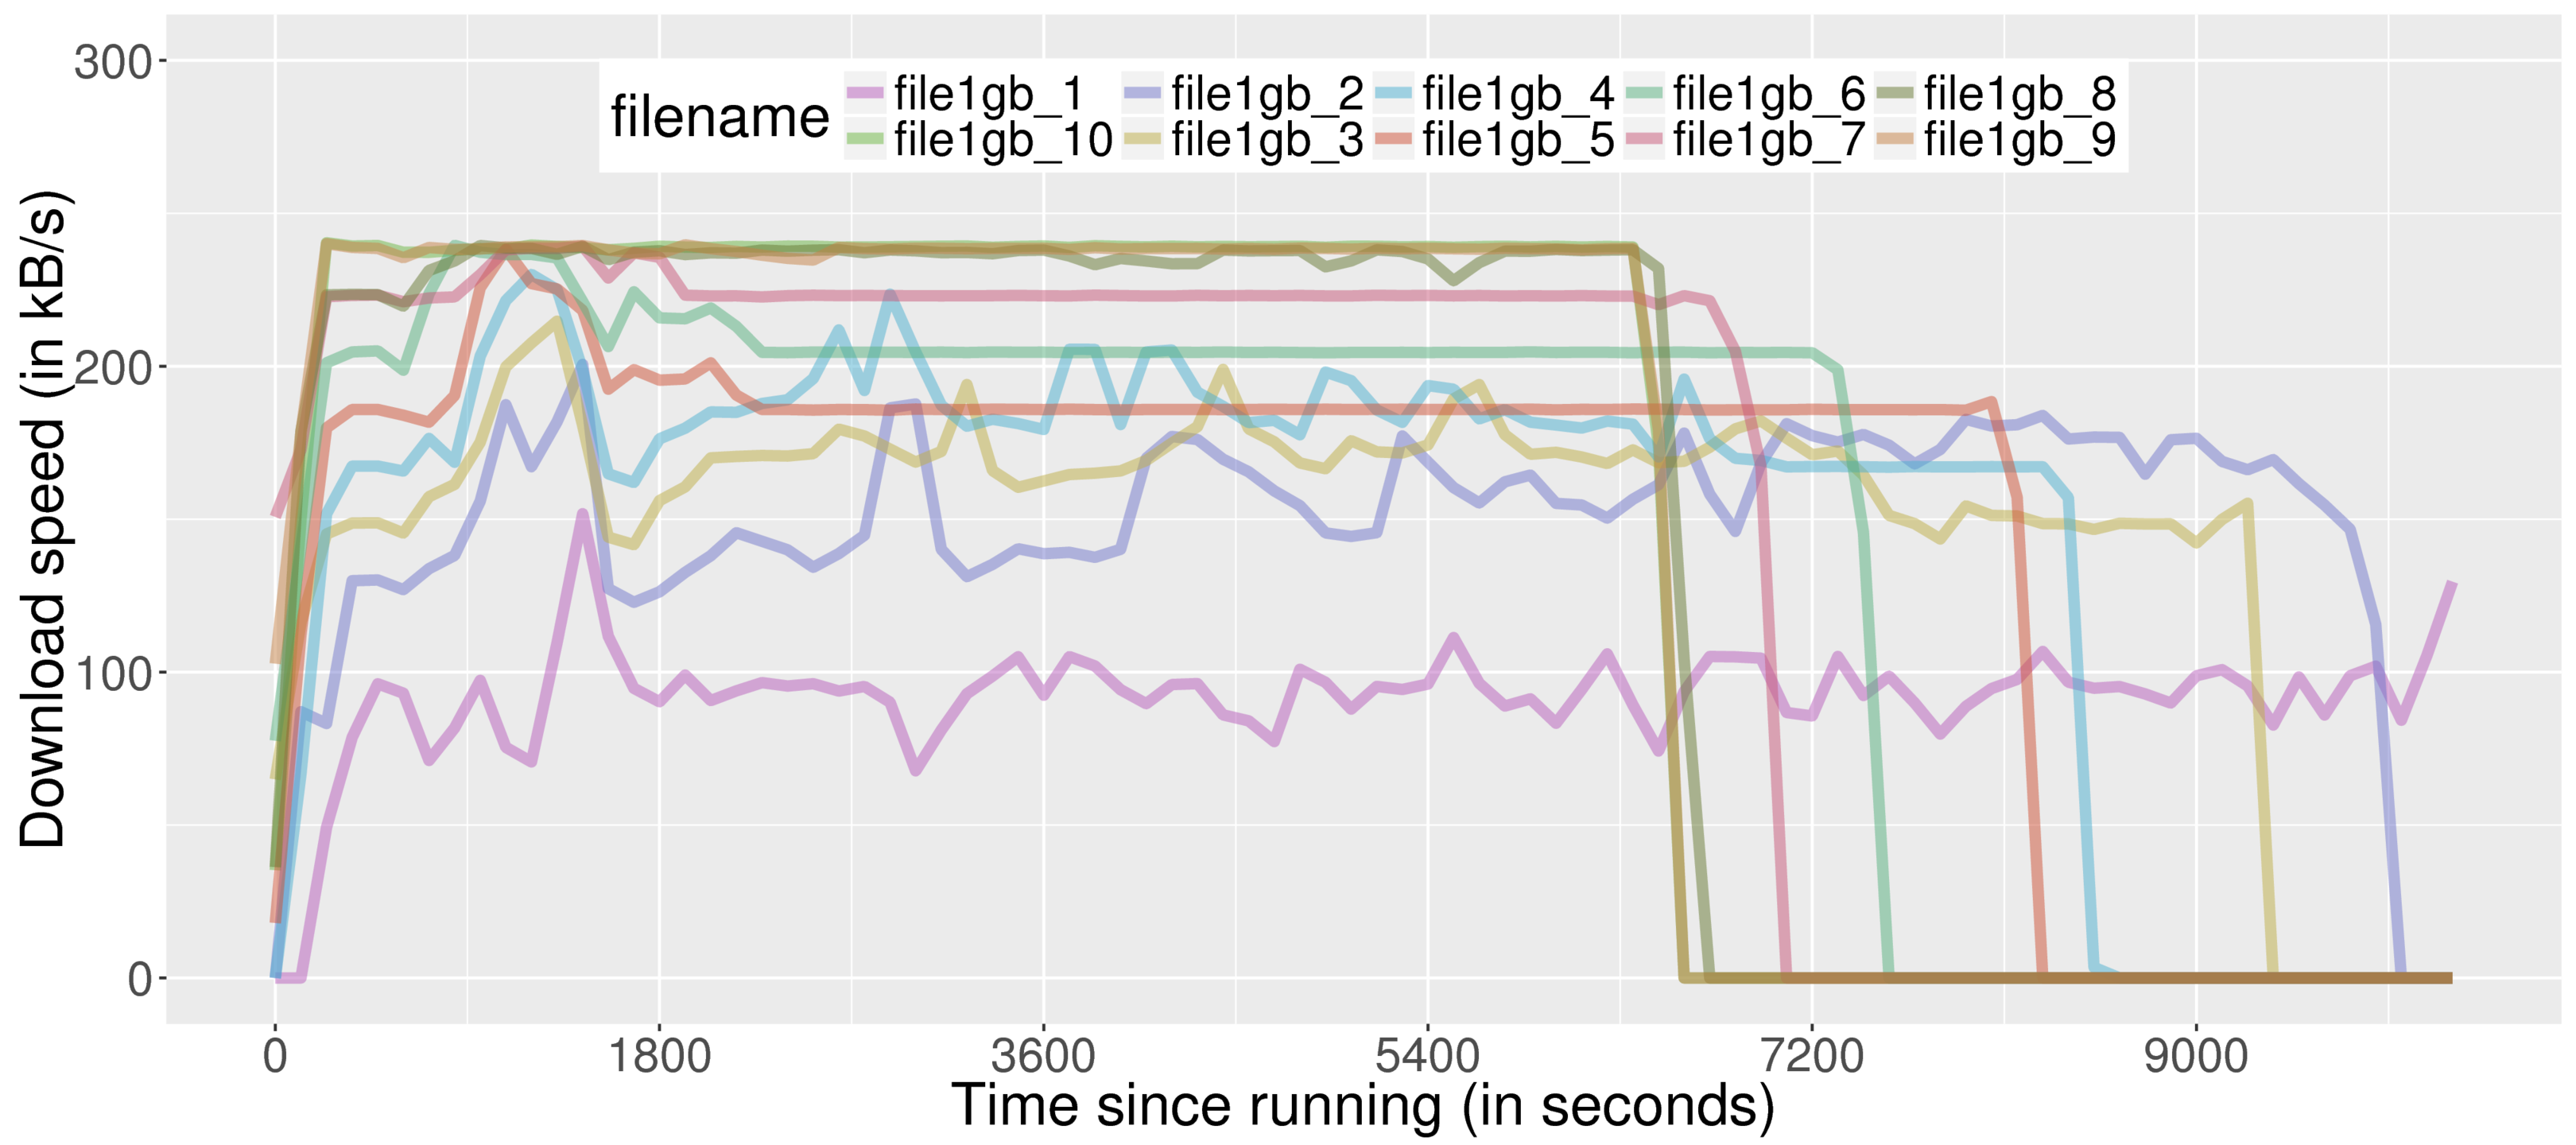
\includegraphics[width=\textwidth]{pics/results/swperf_sc1_10.png}
	\caption{Swarm performance with credit mining in the swarm (10 peers)}
	\label{fig:swarmcm10perf}
\end{figure}

Figure \ref{fig:swarmcm25perfnotrig} : 25 miner without incitement.

\begin{figure}[h!]
	\centering
	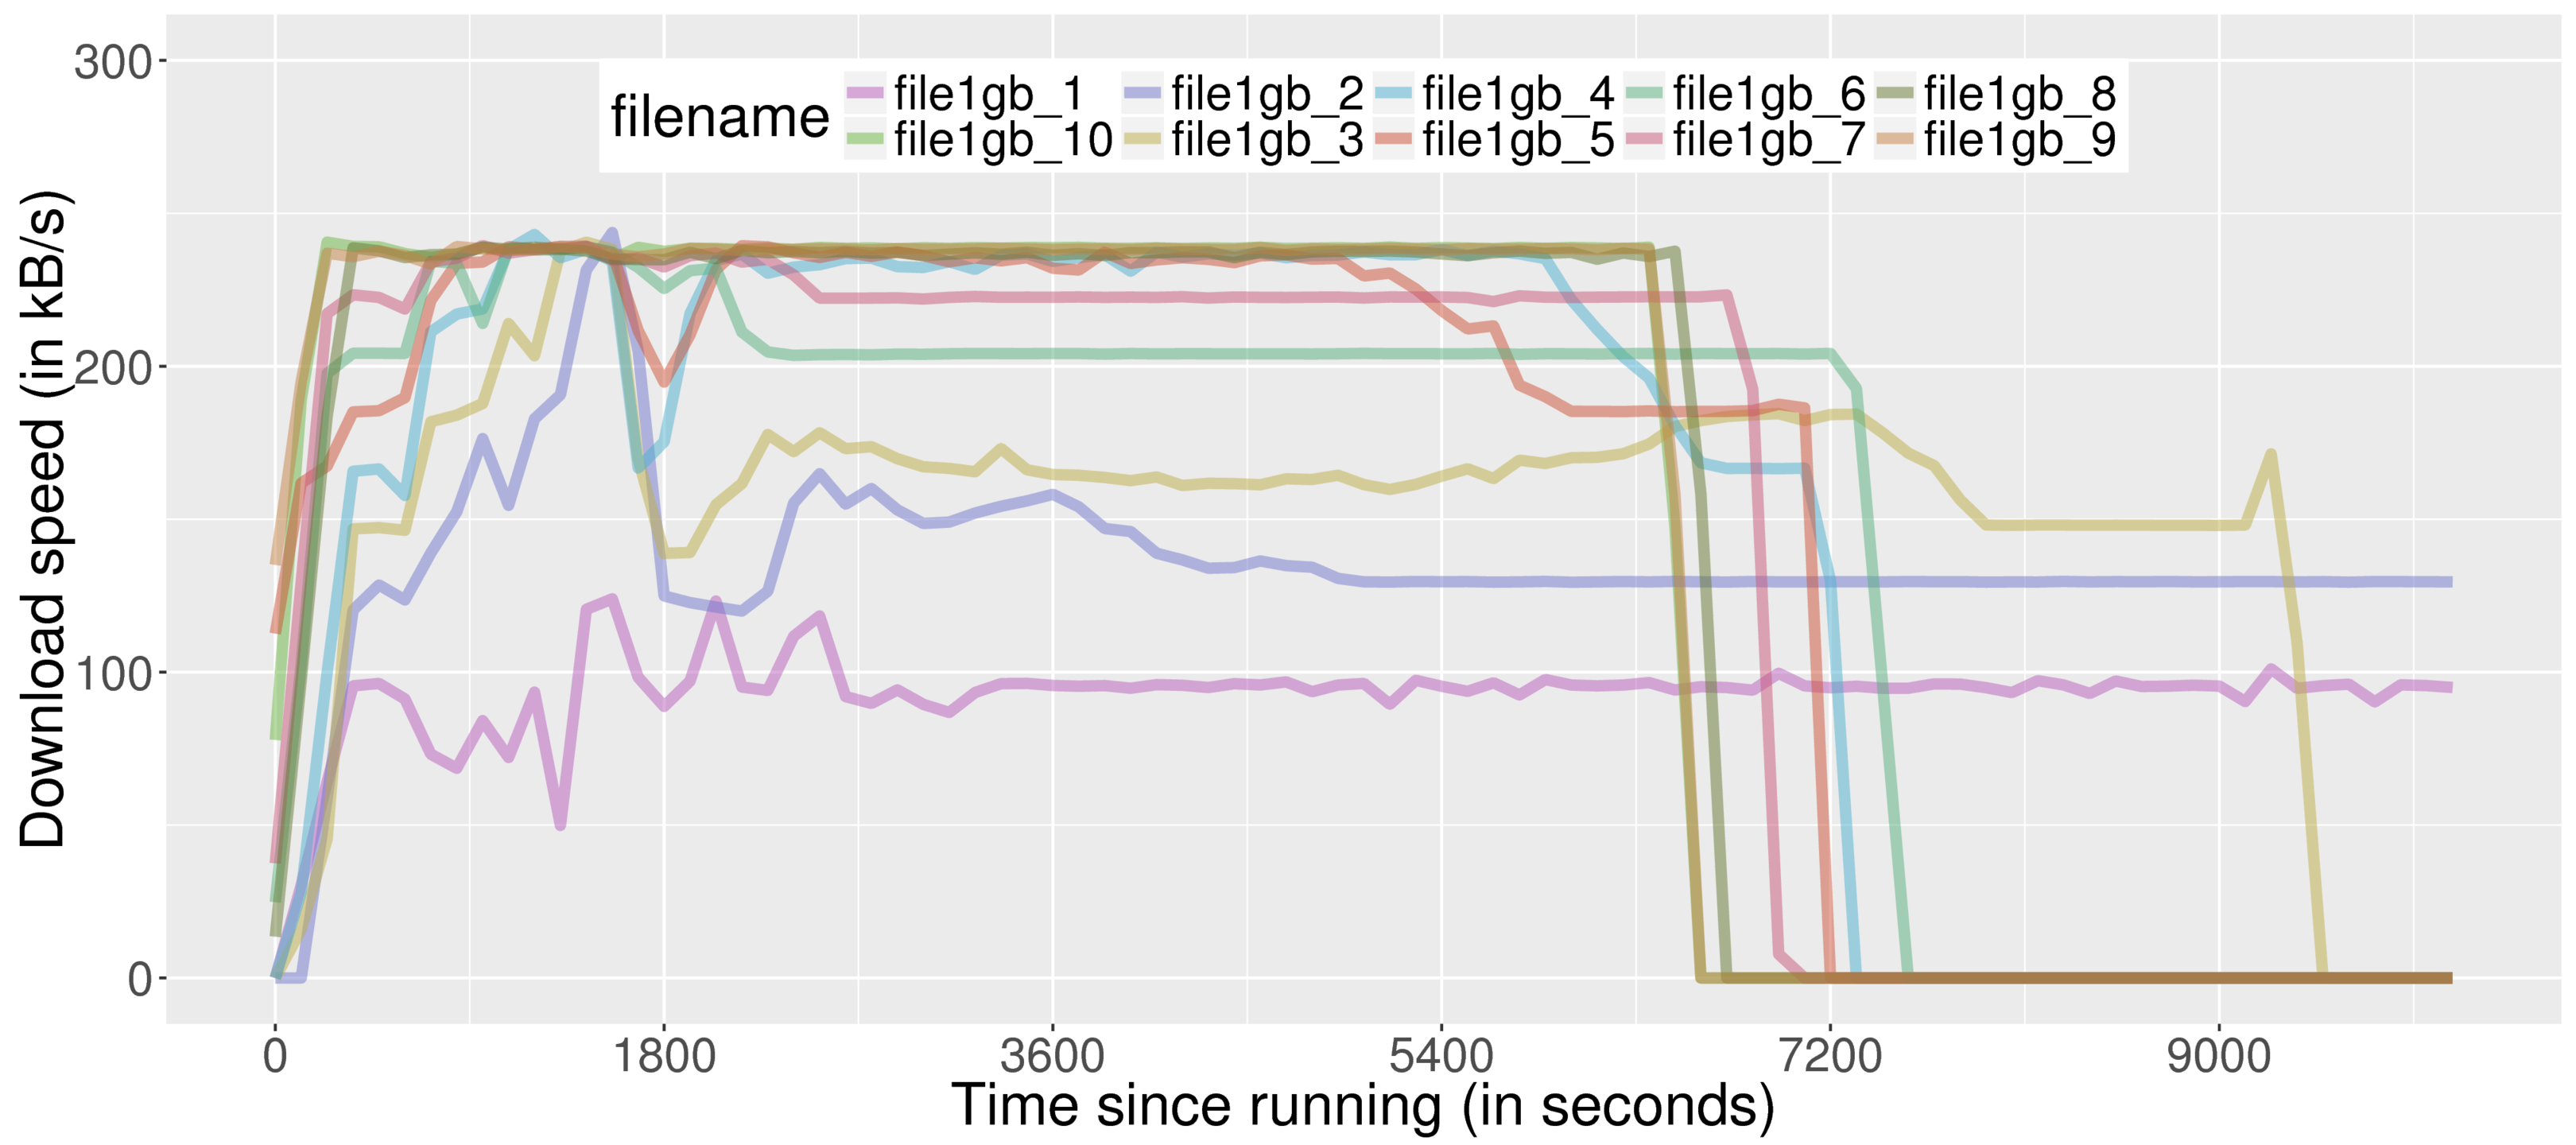
\includegraphics[width=\textwidth]{pics/results/swperf_sc1_notrig.png}
	\caption{Swarm performance with credit mining in the swarm (25 peers) without incitement}
	\label{fig:swarmcm25perfnotrig}
\end{figure}

\clearpage
\subsection{Experiment on user activity}
\todo[inline]{WORK ON PROGRESS - Run experiments. May be dropped}
As mentioned in \ref{section:uactivityimpl}, credit mining system that implemented within Tribler need to accommodate user download activity when mining. This experiment validate that feature by evaluating that there is insignificant effect for user. The expectation is that when both credit mining and user download active, the bandwidth used in user download will keep stable. If only credit mining is active, then it will maximize the bandwidth if possible. For the base data as comparison, the download speed without activating credit mining will be averaged.

The experiment will start in closed environment with 10 nodes. In the scenario, we defined three swarms that available for download. As for node categorization, single node act as a publisher, 7 nodes as seeder, the rest are downloaders. One of the downloader activating credit mining and adding our custom RSS feed as its source. We designed the RSS feed that it will feed relatively popular swarm that easy to mine. The download activity will be started first. Credit mining system will be started in several minutes after that. In the middle of scenario, the downloader stop to download one swarm and then switch to another swarm. We will then compare the download speed of one with credit mining active and one without. 


% #50 -> 25k secs : 7 hour
% #50 -> 12h : 
\begin{figure}[h!]
	\begin{adjustwidth}{-2cm}{}
		\begin{subfigure}[t]{0.6\textwidth}
				\includegraphics[width=\textwidth]{pics/results/prio_act1.png}
				\caption{Download speed of user download activity vs credit mining}
				\label{fig:cmpriomeanagg}
		\end{subfigure}
		~
		\begin{subfigure}[t]{0.6\textwidth}
			\centering
				\includegraphics[width=\textwidth]{pics/results/prio_none.png}
				\caption{Download speed of user download activity only}
				\label{fig:cmpriomean}
		\end{subfigure}
		\caption{Priority figure.}
	\end{adjustwidth}
\end{figure}

%\section{Finding best parameters}
%\label{section:cmparamexp}
%The challenge of designing a configurable system is to know what is the effect of the parameters on its performance. Although in the implementation there are many parameters such as the checking period, blacklist threshold and its recovery time, and number of concurrent active swarm in miners, we focused on one that directly related to prospecting method. Therefore, we ended up with two key parameters that need to be evaluated : scoring policy multiplier and the number of downloaded piece in predownload phase.
%
%The experiments in this category will be conducted in both closed environment and the net. In closed environment, we will compare the properties of the swarm observed. The comparison with base performance where credit mining system is not deployed is performed. On the other hand, when launching in the net, custom RSS feed is used. In this case, our focus will be how the credit mining system gain the credit with provided configuration. Both types of experiment run in DAS 4 for 6 hours with 120 nodes. 
%
%\subsection{Multiplier in scoring policy}
%We have mentioned scoring policy in section \ref{section:prospection}. It works by considering swarm properties then gives a score for the properties. There is a weight/multiplier for each properties that stands for its importance. In this experiment we change the multiplier to find out which property and what weight best represent the swarm for prospecting purpose.
%
%We choose the minimum and maximum multiplier by 1 and 5, respectively. In this experiment, a properties is prioritized when the multiplier is 5. On ther other hand, it is not prioritized when the multiplier is 1. Considering there are three properties that need the multiplier, there are six combinations of prioritizing the properties. The algorithm will be executed for every 1 hour. We take note the swarm it choose and compare it to base experiment. The more swarms that selected correctly, the better multiplier combination define the swarm.
%
%\subsection{Number of piece download}
%Another important point of credit mining system is \textit{predownload} phase. By downloading several pieces in start, we put a capital investment hoping that it will act as a mining catalyst. Intuitively, the more capital investment is placed, the higher return will be gained. However, this is not the case in short or medium period. Moreover, another point of \textit{predownload} also to observe peers to get swarm information. Put a large investment on front may become obsolete in next several round.
%
%We start by disabling the predownload, that is, by set zero as number of piece that need to be predownloaded. Next is by set the number as 4, 20, and 50 to represent few, medium, and many piece, respectively. The number of peer and consumed storage are observed. Then, the chosen swarm that relies on the information generated by \textit{predownload} is noted. To have relatively stable number of peer, we will use custom RSS feed to provide us with old but popular content. 
%\subsection{Peer translation accuracy}